% TODO: you should be using terms flat and tree representation (to match with the documentation)
% TODO: figure out how to make all tables consistently wide across the thesis
% TODO: consistent references (the format of author names, years, pages, etc)

\documentclass[12pt,a4paper,english,twoside,openright]{report}
\usepackage{parskip}

\usepackage[includeheadfoot, inner=3.5cm, outer=3.5cm]{geometry}
\setlength{\headheight}{15pt}

\usepackage{emptypage}
\usepackage{pdfpages}

\usepackage{fancyhdr}
\pagestyle{fancy}
\fancyhf{}
\fancyhead[LE,RO]{\thepage}
\renewcommand{\sectionmark}[1]{ \markright{\thesection\ #1}{} }
\fancyhead[RE,LO]{\rightmark}

\usepackage{adjustbox}
\usepackage{float}
% \floatstyle{boxed}
% \restylefloat{figure}

\usepackage[
  colorinlistoftodos,
  prependcaption,
  textsize=small
]{todonotes}

\usepackage[utf8]{inputenc}
\usepackage[T1]{fontenc,url}
\urlstyle{sf}

\usepackage{siunitx}
\DeclareSIUnit{\nothing}{\relax}
\newcommand{\micros}[1]{\SI{#1}{\micro\second}}
\newcommand{\millis}[1]{\SI{#1}{\milli\second}}
\newcommand{\seconds}[1]{\SI{#1}{\second}}
\newcommand{\kilo}[1]{\SI{#1}{\kilo\nothing}}
\newcommand{\mega}[1]{\SI{#1}{\mega\nothing}}

\usepackage{algpseudocode}
\usepackage{amssymb}
\usepackage{tikz}
\usetikzlibrary{matrix,arrows,backgrounds,fit}

\usepackage{pgfplots}
\usepgfplotslibrary{units}
\usepgfplotslibrary{groupplots}
\pgfplotsset{compat=1.16}

\usepackage{minted}
\newmintinline[ir]{rust}{}
\newmintedfile[rustfile]{rust}{}

\usepackage{babel,textcomp,csquotes,varioref,graphicx}

\usepackage[
  backend=biber,
  maxbibnames=6,
  isbn=false,
  doi=false,
  defernumbers=true
]{biblatex}
\addbibresource{refs.bib}
\setlength\bibitemsep{\baselineskip}

\usepackage[
  pdftitle={Efficient Persistent Vector Implementation for Rust},
  pdfauthor={Araz Abishov},
  hidelinks=true,
  unicode=true  
]{hyperref}
\urlstyle{same}
\usepackage{cleveref}

\raggedbottom

\newcommand{\type}[1]{\emph{\textbf{#1}}}
\newcommand{\crate}[1]{\emph{\textbf{#1}}}

\newcommand{\bigo}[1]{$\mathcal{O}(#1)$}
\newcommand{\bigochar}[1]{$\mathcal{O}$}
\newcommand{\range}[1]{#1}

\newcommand{\pvecrs}{\crate{pvec-rs}}
\newcommand{\imrs}{\crate{imrs}}
\newcommand{\rpds}{\crate{rpds}}
\newcommand{\rayon}{\crate{rayon}}

% Used to refer to the RRB-Tree type 
% provided by pvec-rs.
\newcommand{\rrbtree}{\type{rrbtree}}

% This macro is used to refer to the RRB-Tree 
% as a concept, rather than a concrete type 
% provided by pvec-rs. 
\newcommand{\treerrb}{\emph{RRB-Tree}}

\newcommand{\refcell}{\type{refcell}}
\newcommand{\arc}{\type{arc}}
\newcommand{\rc}{\type{rc}}

\newcommand{\rbtree}{\type{rbtree}}
\newcommand{\rbvec}{\type{rbvec}}
\newcommand{\rrbvec}{\type{rrbvec}}
\newcommand{\pvec}{\type{pvec}}
\newcommand{\imrsvec}{\type{imvec}}
\newcommand{\stdvec}{\type{vec}}

\newcommand{\m}{$m$}
\newcommand{\h}{$h$}
\newcommand{\x}{$x$}
\newcommand{\nil}{\emph{NIL}}
\newcommand{\la}{$\leftarrow$}
\newcommand{\ts}[1]{\textsubscript{#1}}
\newcommand{\n}{\emph{N}}

\algnewcommand\And{\textbf{and}}
\algnewcommand\In{\textbf{in}}

\colorlet{color-path}{blue!30}
\colorlet{color-node}{blue!10}

\definecolor{morange}{HTML}{FF9800}
\definecolor{mpurple}{HTML}{512DA8}
\definecolor{mred}{HTML}{D32F2F}
\definecolor{mgreen}{HTML}{689F38}

\title{Efficient Persistent Vector Implementation for Rust}
\author{Araz Abishov}

\begin{document}

\pagenumbering{roman}
\includepdf[pages={-}]{forside/forside.pdf}
\setcounter{page}{5}

\pdfbookmark[0]{Front matter}{bm-frontmatter}
\pdfbookmark[1]{Contents}{bm-toc}
\tableofcontents{}

\cleardoublepage
\pdfbookmark[1]{List of Listings}{bm-listings}
\listoflistings

\cleardoublepage
\pdfbookmark[1]{List of Figures}{bm-figures}
\listoffigures

\cleardoublepage
\vspace*{2cm}
\thispagestyle{plain}

\phantomsection
\addcontentsline{toc}{section}{Abstract}

\begin{center}
\section*{Abstract}
\end{center}

Rust is a multi-paradigm system programming language focused on performance and reliability. Its rich type system guarantees memory and thread-safety at compile-time.

Rust forbids simultaneous sharing and mutation, that sometimes is a necessary and a useful pattern. A common way to mitigate this limitation in Rust is to clone a value before sharing it. Naive cloning by copying, however, is an expensive operation both in terms of memory and performance.

This thesis presents \pvecrs{}, a project that contributes a vector implementation with efficient clone operation that borrows ideas from persistent data structures. The project explores novel approaches to optimize vector’s performance by leveraging type system of Rust, as well as aiming to achieve convenient, idiomatic interface familiar to developers. The proposed optimizations are evaluated and discussed based on results of the sequential and parallel tests.


\cleardoublepage
\vspace*{2cm}
\thispagestyle{plain}

\begin{center}

\phantomsection
\addcontentsline{toc}{section}{Acknowledgements}

\section*{Acknowledgements}

\end{center}

I would like to thank my supervisors, Martin Steffen and Volker Stolz, for their guidance and feedback. Without their patience and support, as well as trust in my own idea, this venture would not have been possible.

My deepest appreciation goes to my family and my friends for their moral support, their continuous encouragement, and their help whenever it was needed.

Finally, I would like to thank the Rust community for being so welcoming and supportive. In particular, I am grateful to Nicholas D. Matsakis for inspiring me to work on this project.


\cleardoublepage
\thispagestyle{plain}

\begin{center}
    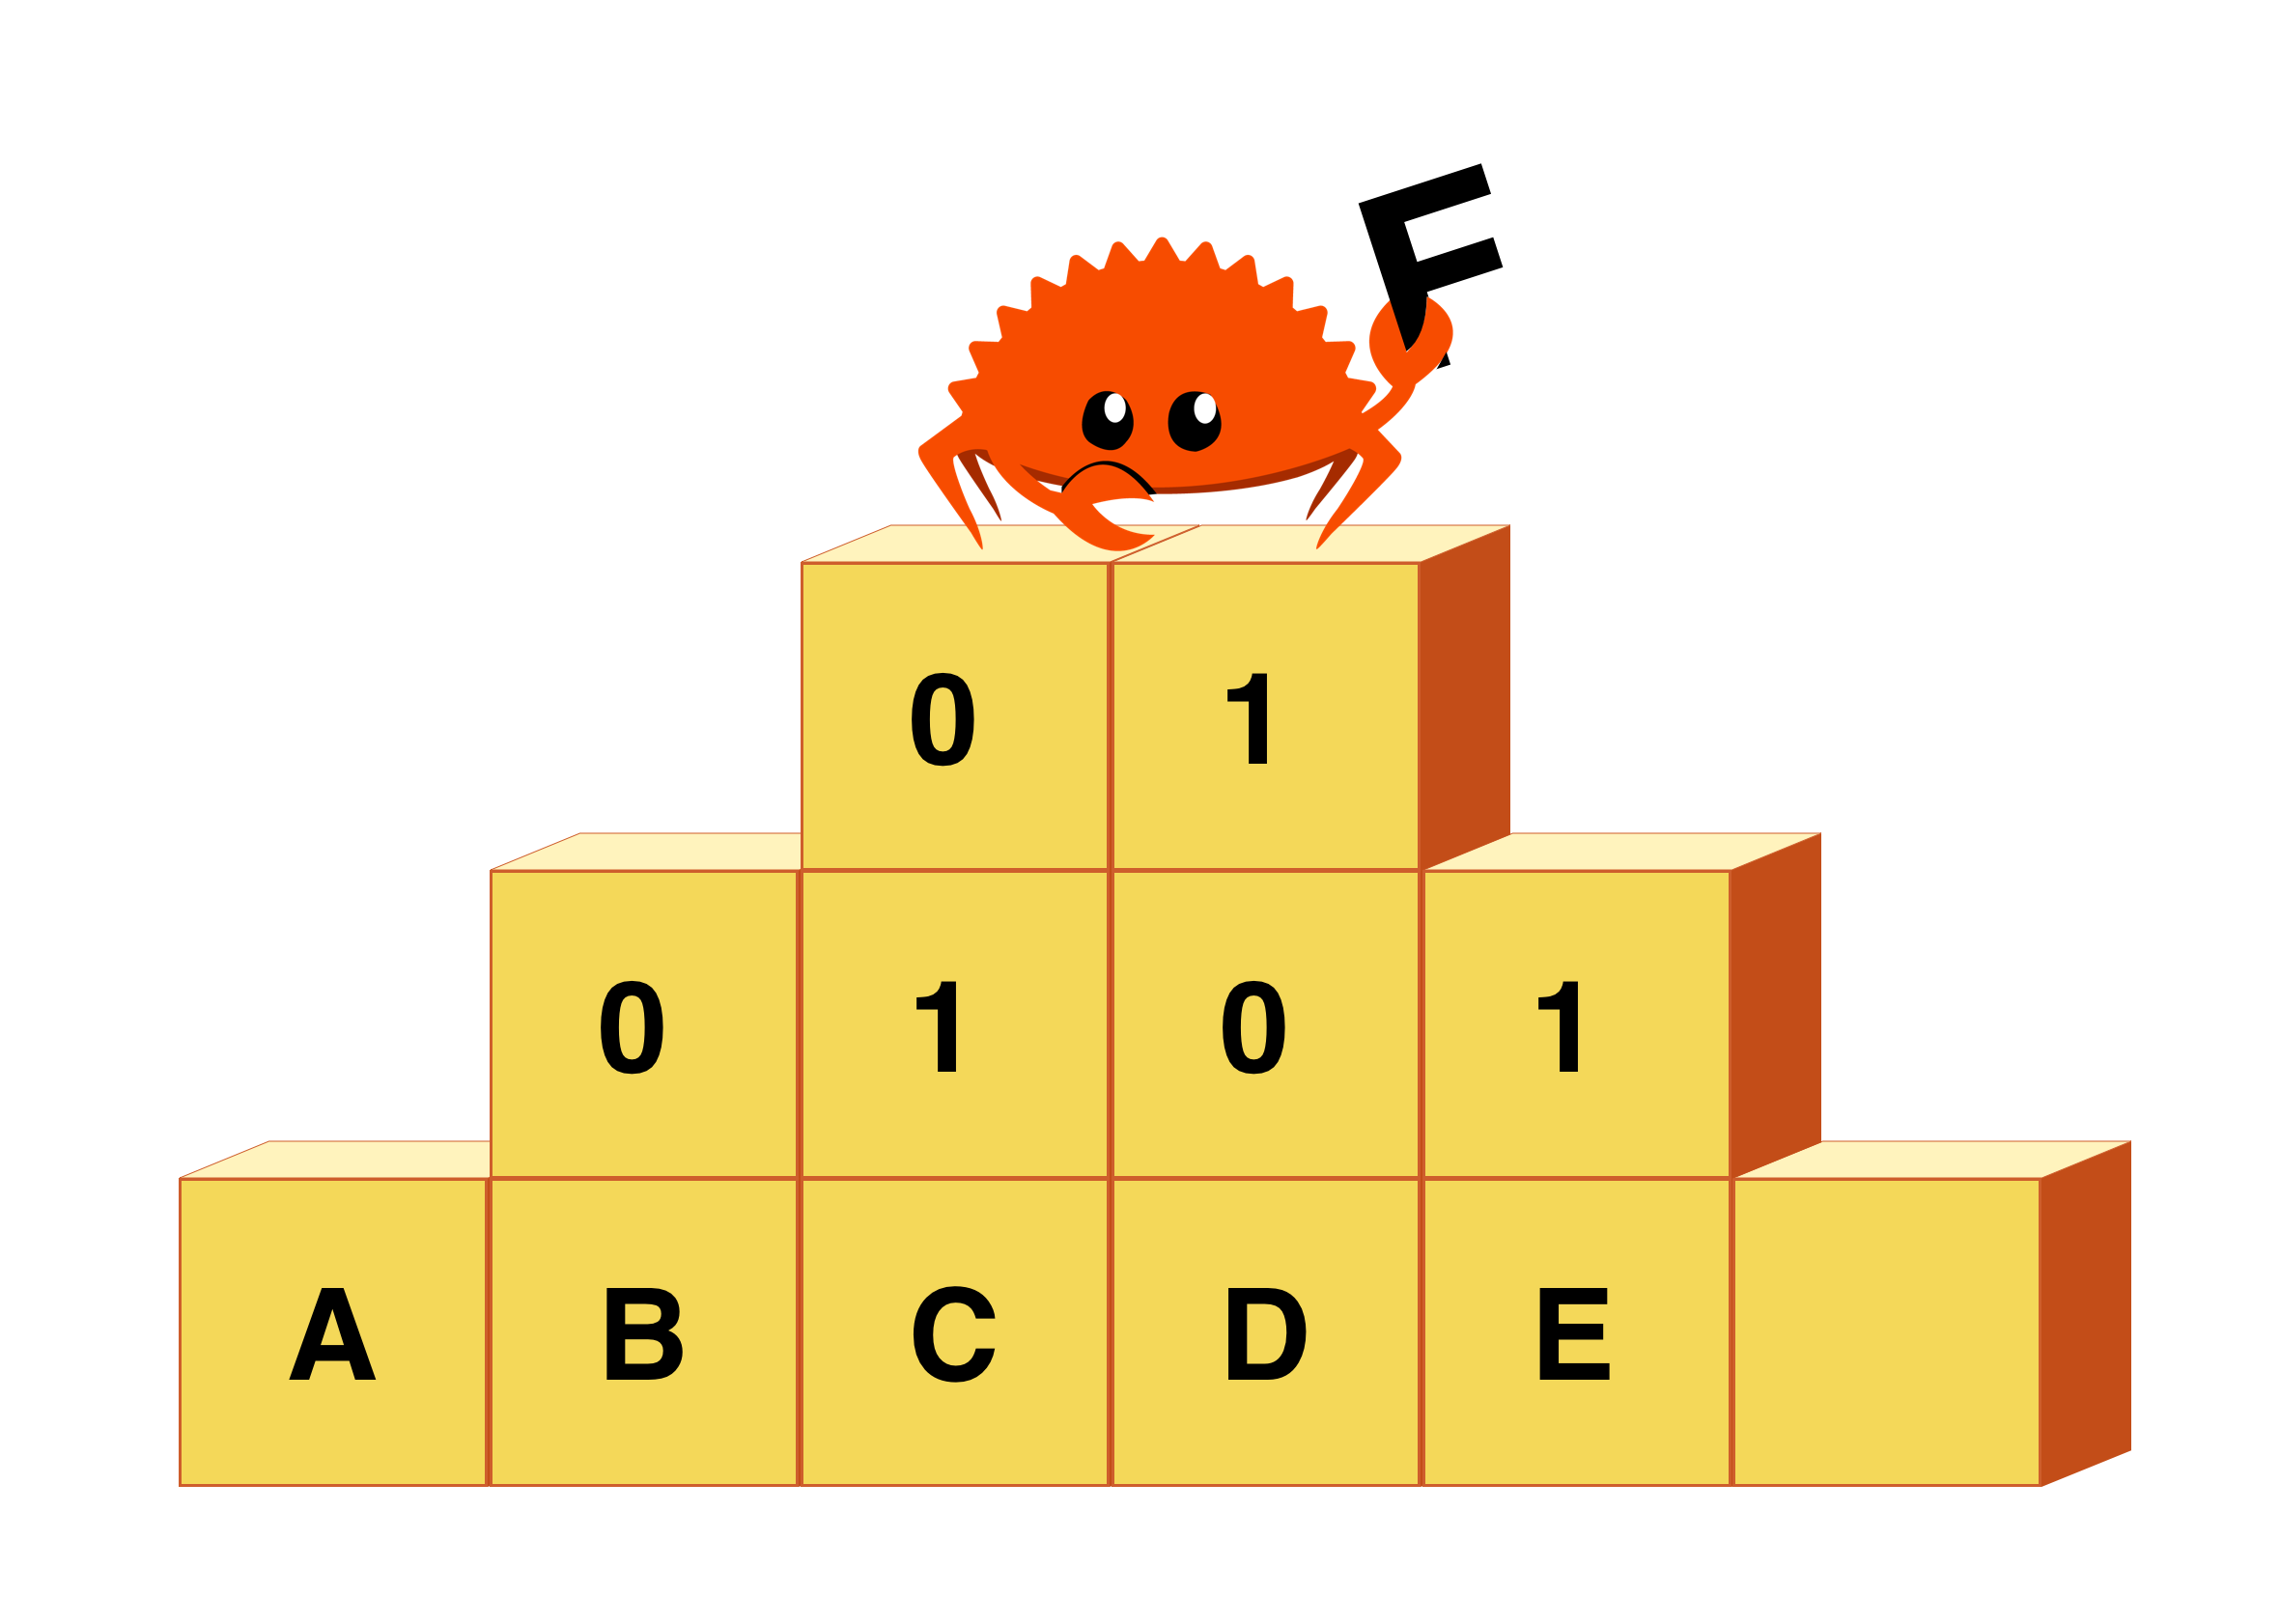
\includegraphics[width=8cm, angle=0, trim=10 10 10 10, clip]{images/ferris-climbing.png}

    \phantomsection
    \addcontentsline{toc}{section}{Reading notes}

    \section*{Reading notes}
    \begin{justify}
        The links to the LaTeX source code and the latest version of this document can be found at \url{https://abishov.com/thesis/}. The implementation, documentation, and visualization demo can be found at \url{https://abishov.com/pvec-rs}.

        If you notice any typos while reading the document, or have any feedback in general, feel free to open an issue at \url{https://github.com/arazabishov/thesis/issues} or send me an email at \href{mailto:araz@abishov.com}{\nolinkurl{araz@abishov.com}}.

        \paragraph{Colophon}
        The illustration above with Ferris\footnote{Unofficial mascot for Rust: \url{https://rustacean.net/}} sitting on top of \treerrb{}, kindly prepared by Vanessa Tesorone. The reading notes design and the idea to use Rust's mascot for the document decoration was inspired by the master's thesis of Erik Vesteraas\footnote{\url{http://erik.vestera.as/thesis/}}.
    \end{justify}

    \subsection*{Typographic conventions}
    \begin{tabular}{ r l }
        Clickable link & \href{https://www.rust-lang.org/}{Rust Programming Language} \\
        Inline code and types & \mintinline{rust}{Vec::new()} \\
        Project or library name & \pvecrs{} \\
    \end{tabular}

\end{center}


\pagenumbering{arabic}

\chapter{Introduction}

% TODO: Optional<Add a point to introduction to describe what is RefCell>
% TODO: Linear types (from Jean's work):
% Earlier work has lead to the definition of linear types, a way to define mutable types in a similar fashion as transients, with focus on correctness [20]. A linear type can only be used once, although relaxed constraints provide means to temporarily define a linear type as nonlinear, which gives users read capabilities without “using” the instance. In contrast, a transient is an affine type, where the function persistent! converts the affine nodes permanently to nonlinear, persistent nodes. 
% TODO: Linear types can change the world

\section{Persistent data structures}

A vast majority of modern programming languages are equipped with a standard library --- a set of constructs and utilities aimed to improve the developer's productivity. 

A significant part of standard library consists of commonly used data structures such as lists, sets, and maps, which often provide operations for reading and writing data. 

Modifying or \emph{mutating} an \emph{ephemeral} data structure implies that we no longer will have access to its older version. In contrast, a \emph{persistent} data structure allows access to any version, old or new, at any time \cite{making-data-structures-persistent}. 

Persistent data structures could be classified based on the operations which they offer over their versions:
\begin{itemize}
    \item \textit{Partial persistence} --- In this persistence model, we can query any previous version of the data structure, but we can update only the newest version. The versions are linearly ordered. 
    \item \textit{Full persistence} --- Both access and updates are allowed on all versions. The versions can be visualized as a branching tree.
    \item \textit{Confluent persistence} --- In addition to the previous operations, it offers combination operation to merge more than one previous version to output a new single version. The versions form a directed acyclic graph \cite{fully-persistent-lists-with-catenation}.  
    \item \textit{Functional persistence} --- This model takes its name from functional programming where objects are immutable. In comparison to the previous models, it prohibits change of the internal representation of the data structure \cite{purely-functional-data-structures}. 
\end{itemize}

While persistence can be achieved by simple copying, the performance of a modification operation quickly becomes unacceptable. This led to research and development of more efficient solutions, which were often designed to solve particular problems. A lack of general purpose collections, which guarantee uniformly good performance across different operations, results in challenges with software development. 

A persistent \emph{vector}, also known as a one-dimensional growable array, is very inefficient if implemented naively. Each update operation will cause a full copy of the underlying array, consuming additional amount of memory and processor time. 

However most operations modify only some parts of data structures, a complete copy is redundant. A better approach is to exploit the similarity between the new and old versions by \emph{sharing} structure between them. For example, instead of representing a data structure as a single block of memory, it could be broken down into smaller pieces or \emph{nodes}, which are linked together in the form of a \emph{tree}. Since modifications only apply to some nodes, the rest of them still remain unchanged and can be shared without copying. 

The first persistent vector implementation which offered good performance across a broad range of operations was introduced by Rich Hickey in the Clojure programming language. It was based on Phil Bagwell's Hash Array Mapped Trie \cite{ideal-hash-trees}, which offers practically constant runtime for push, update, and access operations, and it is a \emph{fully} persistent data structure. 

Later Phill Bagwell introduced a confluently persistent vector based on Relaxed Radix Balanced Tree \cite{efficient-immutable-vectors}, which has improved performance of the concatenation operation significantly and became a foundation for Scala's standard library vector implementation. 

The project presented in the thesis contributes an efficient persistent vector implementation for Rust based on Relaxed Radix Balanced Tree, which takes advantage of the Rust's type system to improve performance, guarantee thread safety and provide an idiomatic application programming interface. In order to ensure the best possible average performance, its internal representation switches from standard vector to RRB-Tree during runtime. 

\section{The Rust programming language}
\todo{The Rust programming language}

\subsection{Ownership and borrowing}
\todo{Ownership and borrowing}

\subsection{Reference counting and memory management}
\todo{Reference counting and memory management}

\section{Contributions}
\todo{Contributions}

\chapter{Radix Balanced Tree}

Radix Balanced Tree or \emph{\rbtree}, is a tree like data structure where each node has at most \m{} number of children and uses element indices as keys. It was first introduced by Rich Hickey as a basis for the persistent vector implementation in the Clojure's standard library \cite{the-clojure-programming-language}. 

Most data structures are tailored to specific use cases, with some operations being faster than others. For example, a persistent linked list can prepend elements and read the head in \bigo{1} time. However, random access is proportional to \bigo{n}, which is unacceptable in practical scenarios. 

In comparison, the Clojure's vector implementation is delivering \emph{practically} \bigo{1} time on fundamental operations such as access, update, push, and pop, rivaling ephemeral vector in performance.

This chapter introduces the inner workings of \rbtree{} and covers algorithms used in core operations. For more formal description of the persistent vector refer to \cite{improving-performance-through-transience}. 

\section{Memory layout}
\label{sec:rb-tree-memory-layout}

\rbtree{} consists of nodes which contain references either to other sub-trees or values. We will be calling the former type of node as \emph{branch} node, while the latter one as \emph{leaf}. The number of sub-trees and values in the node is configurable and will be denoted as \m{}, also known as \emph{branching factor}. 

When \m{} is set to a large value, \rbtree{} becomes wide and shallow. In practice, the branching factor is set to 32 to achieve \emph{practically} \bigo{1} performance across different operations, but technically this number can be any power of 2.

From now and onwards the height of the tree will be referred to as \h{}. The upper bound of \h{} can be calculated using ${\log_m(n - 1) + 1}$, where $n$ is the total count of elements in the tree. If \m{} is 32 and the number of elements will never be larger than the maximum index representable with 32 bit signed integers, the maximum height of the tree won't exceed 7 levels. 

References to values are stored at the leaf nodes of the tree. If the count of values stored in the structure is less than branching factor, then the root node itself will be a leaf. Otherwise, capacity of the tree is increased by adding intermediate, branch nodes, which contain references to other branches or leaves. 

\section{Radix search}

Before trying to understand how primitive operations such as push, pop and update work, let's take a look at how to access the right element in \rbtree{}. The lookup mechanism is called \emph{radix search}, a fundamental operation which forms the basis for other primitives.

Conceptually, the idea behind search in a tree-like structure boils down to picking correct nodes based on the given key. If there is a value corresponding to the key, we stop searching and return the value. Otherwise, an empty value or error is returned.

The lookup mechanism often depends on organization of nodes in the tree. Let's consider an example where each node can have at most two child nodes, called \emph{binary tree}. A binary tree where every node fits a specific ordering property is called \emph{binary search tree}. While searching, the key at each node is compared to the search key. All that is important is whether the key in the node is less than, equal to, or greater than the search key. The search is continued until an exact match or reaching leaf nodes.

Another tree-like data structure --- trie, also known as prefix tree, is interesting because its nodes do not store complete keys. Instead, each node stores only part of it. A trie is a variant of an n-ary tree in which characters are stored at each node. Each path down the tree may represent a word. A node in a trie could have anywhere from 0 through the size of the alphabet children. For example, English alphabet has 26 letters, meaning that each node in a trie might have up to 26 children.

The lookup procedure for tries involves breaking down the search key into multiple sub-keys, which are used to pick corresponding sub-tries. For example, the key "car" will be broken down into several smaller keys such as "c", "a", "r". If there is a value present at the last node of the path, it is returned. Otherwise, the search key is not present in the structure.

\subsection*{Bit partitioning}

\rbtree{} is a variation of a trie, which is also known as \emph{persistent bit-partitioned vector trie}. So what does make it so special? 

A search key in \rbtree{} is an integer, which can be viewed as a composite key, where each sub-key is represented by a sequence of bits. The idea is to divide the key into blocks of bits, where each block forms an index specific to the tree node. The count of bits in each of those chunks can be derived from the branching factor and will be called as \emph{bits per level}.

The \emph{bits per level} or \x{} is the count of bits used to address \m{} nodes in the binary numeral system. The relationship between \m{} and \x{} can be represented as: 

\begin{equation}
    2^x = m
\end{equation}

This leads us to a formula which derives the count of \emph{bits per level} from \m{}: 

\begin{equation}
    \label{eq:bits-per-level}
    x = log_2(m)
\end{equation}

For example, with \m{} equal to 16, the maximum index value is 15. 15 converted to the binary form is $1111_2$, which evidently requires 4 bits of space. If we substitute \m{} into \Cref{eq:bits-per-level}, we will get the same value. 

\subsection*{Extracting sub-keys}

Now when the size of the sub-key is known, next step is to identify its location. The count of sub-keys within the search key depends on the heght of the tree. Each new level in \rbtree{} will use \x{} additional bits of space. For instance, a search key addressing an element of the tree of ${h = 3}$ and ${x = 2}$ will consist of 3 sub-keys taking up 6 bits of space in total.

Sub-keys are arranged in the order from the most to the least significant bits, where the most significant sequence is a key used to access child node of the root. Each following key is used to index into child node on the corresponding tree level.

Knowing the depth at which a node is located and the count of bits per level, the value of the key can be calculated using bitwise operations such as logical shift and masking. Let's take a look at mechanism used to extract the right sub-key. 

In the following example there is a byte which represents a key equal to 54. Let's assume that it belongs to the tree where \m{} is 4, \x{} is 2 and that height of the tree 3. 

\begin{equation}
    54_{10} = 00110110_2    
\end{equation}

Since there are three levels, we have only three sub-keys: $11_2$, $01_2$ and $10_2$. Let's say that we are interested in extracting sub-key for the child node on the second level --- $01_2$. 

First, let's get rid of the bits following the sub-key of our interest. Logical right shift operation --- $\ggg$, will push $(l - 1) * x$ 0s into key, where $l$ is the \emph{level} at which current node is located. 

\begin{equation}
    00110110 \ggg ((l - 1) * x)
\end{equation}

Since the node in the example is located at $l = 2$ and $x = 2$, the search key will be shifted by 2. The result of operation is $00001101_2$. As you can see, the "tail" of the key is truncated.

The next step is to get rid of bits preceding the sub-key by masking them to 0. An operator used for this is known as bitwise "and" and it will be applied to the result of shifting operation. 

A bitwise "and" takes two equal-length binary representations and performs the logical "and" operation on each pair of the corresponding bits. 

Thus, if both bits in the compared position are 1, the bit in the resulting binary representation is 1; otherwise, the result is 0. Here is an example:

\begin{equation}
    00001101 \ \& \ 00000011 = 00000001
\end{equation}
                                    
The first and the second operands are the key and mask respectively. 

Only the last two bits of the mask are set to 1, which means that all bits of the key except last two will be masked to 0. The result of the "and"-ing operation will be the value of the sub-key.

Now the question is how to define a mask and what are the requirements to it. First of all, it has to be of the same type as the key, meaning that it must have the same count of bits in the binary representation. Secondly, the last \x bits must be set to 1.

The mask is equal to the maximum value of the sub-key, which can be calculated from the branching factor:

\begin{equation}
    mask = m - 1
\end{equation}

If \m{} is equal to 4 the maximum sub-key value will be 3, which equals to 00000011 in the binary representation.

\subsection*{Summary}

\begin{figure}        
    \caption{Accessing element at index 104 in a tree of height 4. Empty nodes represent collapsed subtrees.}
    \label{fig:rb-tree-example-1}

    \centering
    \begin{tikzpicture} [    
        node/.style = { 
            matrix of nodes, 
            nodes = { draw, minimum width = 6mm, minimum height = 8mm, anchor = center},
            font = \small,
            nodes in empty cells        
        },    
        value/.style = { 
            matrix of nodes, 
            nodes = { draw = none, minimum width = 4mm, minimum height = 4mm, anchor = center, rotate = 90 },
            font = \small,            
            nodes in empty cells        
        },    
        edge/.style = { ->, shorten >= 4pt }
    ]   
        \node[] (index) at (current page.north west) { $104_{10}$ = $01 10 10 00_{2}$ };        
        
        \matrix[node] (node-1-1) [below right = 8mm and 1cm of index] { 00 & 01 & 10 & 11 \\ };
                
        \scoped[on background layer] {
            \node[fit=(node-1-1-1-1), fill=color-node, inner sep = 0pt]   {};
            \node[fit=(node-1-1-1-2), fill=color-path, inner sep = 0pt]   {};
            \node[fit=(node-1-1-1-3), fill=color-node, inner sep = 0pt]   {};
            \node[fit=(node-1-1-1-4), fill=color-node, inner sep = 0pt]   {};
        }
        
        \matrix[node, inner sep = 0pt] (node-2-2) [below left = 8mm and 1mm of node-1-1.south] { 00 & 01 & 10 & 11 \\ };
        \matrix[node, fill = color-node, inner sep = 0pt] (node-2-3) [below right = 8mm and 1mm of node-1-1.south] { & & & \\ };
        \matrix[node, fill = color-node, inner sep = 0pt] (node-2-1) [left = 2mm of node-2-2.west] { & & & \\ };
        \matrix[node, fill = color-node, inner sep = 0pt] (node-2-4) [right = 2mm of node-2-3.east] { & & & \\ };

        \scoped[on background layer] {
            \node[fit=(node-2-2-1-1), fill=color-node, inner sep = 0pt]   {};
            \node[fit=(node-2-2-1-2), fill=color-node, inner sep = 0pt]   {};
            \node[fit=(node-2-2-1-3), fill=color-path, inner sep = 0pt]   {};
            \node[fit=(node-2-2-1-4), fill=color-node, inner sep = 0pt]   {};
        }

        \draw[edge, out=225, in=45] (node-1-1-1-1.south) to (node-2-1.north);
        \draw[edge, out=225, in=45] (node-1-1-1-2.south) to (node-2-2.north);
        \draw[edge, out=315, in=135] (node-1-1-1-3.south) to (node-2-3.north);
        \draw[edge, out=315, in=135] (node-1-1-1-4.south) to (node-2-4.north);

        \matrix[node, fill = color-node, inner sep = 0pt] (node-3-2) [below left = 8mm and 1mm of node-2-2.south] { & & & \\ };
        \matrix[node, inner sep = 0pt] (node-3-3) [below right = 8mm and 1mm of node-2-2.south] { 00 & 01 & 10 & 11 \\ };
        \matrix[node, fill = color-node, inner sep = 0pt] (node-3-1) [left = 2mm of node-3-2.west] { & & & \\ };        
        \matrix[node, fill = color-node, inner sep = 0pt] (node-3-4) [right = 2mm of node-3-3.east] { & & & \\ };

        \scoped[on background layer] {
            \node[fit=(node-3-3-1-1), fill=color-node, inner sep = 0pt]   {};
            \node[fit=(node-3-3-1-2), fill=color-node, inner sep = 0pt]   {};
            \node[fit=(node-3-3-1-3), fill=color-node, inner sep = 0pt]   {};
            \node[fit=(node-3-3-1-4), fill=color-path, inner sep = 0pt]   {};
        }

        \draw[edge, out=225, in=45] (node-2-2-1-1.south) to (node-3-1.north);
        \draw[edge, out=225, in=45] (node-2-2-1-2.south) to (node-3-2.north);
        \draw[edge, out=315, in=135] (node-2-2-1-3.south) to (node-3-3.north);
        \draw[edge, out=315, in=135] (node-2-2-1-4.south) to (node-3-4.north);

        \matrix[node, fill = color-node, inner sep = 0pt] (node-4-2) [below left = 8mm and 1mm of node-3-3.south] { & & & \\ };        
        \matrix[node, fill = color-node, inner sep = 0pt] (node-4-3) [below right = 8mm and 1mm of node-3-3.south] { & & & \\ };
        \matrix[node, fill = color-node, inner sep = 0pt] (node-4-1) [left = 2mm of node-4-2.west] { & & & \\ };        
        \matrix[node, inner sep = 0pt] (node-4-4) [right = 2mm of node-4-3.east] { 00 & 01 & 10 & 11 \\ };

        \scoped[on background layer] {
            \node[fit=(node-4-4-1-1), fill=color-path, inner sep = 0pt]   {};
            \node[fit=(node-4-4-1-2), fill=color-node, inner sep = 0pt]   {};
            \node[fit=(node-4-4-1-3), fill=color-node, inner sep = 0pt]   {};
            \node[fit=(node-4-4-1-4), fill=color-node, inner sep = 0pt]   {};
        }
        
        \draw[edge, out=225, in=45] (node-3-3-1-1.south) to (node-4-1.north);
        \draw[edge, out=225, in=45] (node-3-3-1-2.south) to (node-4-2.north);
        \draw[edge, out=315, in=135] (node-3-3-1-3.south) to (node-4-3.north);
        \draw[edge, out=315, in=135] (node-3-3-1-4.south) to (node-4-4.north);

        \matrix[value] (node-5-1) [below = 0mm of node-4-1.south] { 139 & 140 & 141 & 142 \\ };
        \matrix[value] (node-5-2) [below = 0mm of node-4-2.south] { 143 & 144 & 145 & 146 \\ };
        \matrix[value] (node-5-3) [below = 0mm of node-4-3.south] { 147 & 148 & 149 & 150 \\ };
        \matrix[value] (node-5-4) [below = 0mm of node-4-4.south] { 151 & 152 & 153 & 154 \\ };
    \end{tikzpicture}
\end{figure}

Let's put everything together and review the radix search step by step based on the concrete example. In \Cref{fig:rb-tree-example-1}, we can see a part of the \rbtree{} which represents elements of persistent vector in the range [92, 107].

The branching factor of the tree is equal to 4, which means that 2 bits will be used for the sub-key representation. The mask is equal to 3 or 00000011 in the binary representation.

The index type is \emph{unsigned byte}, which has a capacity of 256 \footnote{The capacity of any integer type can be calculated by taking the base of the system --- 2, to the power of bits available for its representation. For byte, it will be $2^8 = 256$.}. In practice, the index type is usually a 32 or a 64 bit integer, which has significantly bigger capacity.

The height of the tree in the given state is 4. The node at the top is root, while nodes at the bottom are leaves. The goal is to lookup the contents of an element corresponding to the key 104. 104 in binary representation is equal to 01101000.

Here are the steps which outline the radix search algorithm for the given example: 
\begin{itemize}
    \item Set node and level variables to root and $h - 1$ correspondingly.
    \item As level is bigger than 0, the for loop will be entered:
    \begin{itemize}
        \item Shift the key by $level * x$ bits: $104 \ggg 6 = 00000001_2$.
        \item Mask the result of previous operation: $00000001\ \& \ 00000011 = 00000001$, which yields the sub-key equal to $1_{10}$.
        \item The node is replaced with the child node at index 1. 
    \end{itemize}
    \item Level is decremented by 1 and now equals to 2. 
    \item As level is bigger than 0, the for loop will be entered: 
    \begin{itemize}
        \item Shift the key by $level * x$ bits: $104 \ggg 4 = 00000110_2$.
        \item Mask the result of previous operation: $00000110\ \& \ 00000011 = 00000010$, which yields the sub-key equal to $3_{10}$.
        \item The node is replaced with the child node at index 3.
    \end{itemize}
    \item Level is decremented by 1 and now equals to 1. 
    \item As level is bigger than 0, the for loop will be entered: 
    \begin{itemize}
        \item Shift the key by $level * x$ bits: $104 \ggg 2 = 00011010_2$.
        \item Mask the result of previous operation: $00011010\ \& \ 00000011$, which yields the sub-key equal to $3_{10}$.        
        \item The node is replaced with the child node at index 3.
    \end{itemize}
    \item Level is decremented by 1 and now equals to 0. 
    \item As level is no longer bigger than 0, we exit the for loop.
    \item Perform masking over the key: $01101000\ \& \ 00000011 = 00000000$, which yields the sub-key equal to $0_{10}$.
    \item Return the value at node of index 0 --- 151.    
\end{itemize}

\begin{listing}[ht!]        
    \caption{Pseudocode for the RB-Tree's radix search implementation}
    \label{lst:rb-tree-radix-search}

    \begin{algorithmic}
        \Function{RadixSearch}{root, key}
            \State $node \leftarrow root$

            \For{$level \leftarrow root_{height} - 1, 1$}
                \State $index \leftarrow (key \ggg (level * x))\ \&\ mask$
                \State $node  \leftarrow node[index]$
            \EndFor

            \State $index \leftarrow key\ \&\ mask$
            \State \Return ${node[index]}$
        \EndFunction
    \end{algorithmic}
\end{listing}

\section{Update}
The purpose of the update operation is to replace the value in the instance of \rbtree{} for the given search  key. 

\emph{Emphemeral} update is \emph{destructive}, meaning that the original \emph{version} of the data structure will be no longer available after the operation is executed. For \emph{persistent data structures}, update results in the new \emph{version} including the updated value without the original becoming unavailable. 

\emph{Version} is something what differentiates one instance of the \rbtree{} from another. Instead using an explicit versioning such as assigning unique numbers to instances of \rbtree{}, we will rely on the memory address as unique identifier. 

The update function accepts two arguments: a search key and a new value. If operation is successfully executed, It returns a new instance of \rbtree{}. If the search key is not present in the original version, new value is either ignored or error is returned. 

There are a few challenges associated with the implementation. If radix search was only reading values without any modifications, update is supposed to both change the value for the given key and ensure that the original structure stays unmodified. 

\subsection*{Path copying}
Radix search will be used to find the value corresponding to the given key. In order to make sure that original data structure is not modified, each branch and leaf node on the way from the root to the value will be copied. This process is also know as \emph{path copying} \cite{planar-point-location}. It is important to emphasize that nodes which are not a part of the path are reused, instead of being recreated. 

In order to get a sense of how well path copying performs, let’s review the whole process in reverse. The leaf node update creates a copy of underlying array of size \m{}. Then, the \m{} sized parent branch node is copied as well, where the fresh copy of the leaf is used instead of the original. The other children of the parent are reused. The same process applies to the grand parent and so on all the way up to the root.  

To summarize, the update operation performs the \h{} count copies of \m{} sized nodes, where \h{} is the maximum height of the tree. As described in \Cref{sec:rb-tree-memory-layout}, \h{} is bound by \bigo{log_m(n)}, which results in the {\bigo{m * log_m(n)}} complexity of the update operation. 

When branching factor \m{} is set to a large value such as 32, performance becomes \bigo{1} in practice. For example, if the tree was completely full, where the count of all elements $n$ is bound by the maximum value of 32 bit integer —  2147483647, \h{} will be at most 7. Since both \h{} and \m{} are effectively constant factors, the resulting performance is proportional to \bigo{1}. 

\begin{listing}[ht!]        
    \caption{Pseudocode for the RB-Tree's update implementation}
    \label{lst:rb-tree-update}
    
    \begin{algorithmic}
        \Function{Update}{root, key, value}
            \State $newRoot \leftarrow clone(root)$
            \State $node \leftarrow newRoot$
    
            \For{$level \leftarrow root_{height} - 1, 1$}
                \State $index \leftarrow (key \ggg (level * x))\ \&\ mask$
                \State $newChildNode \leftarrow clone(node[index])$
                \State $node[index] \leftarrow newChildNode$
                \State $node \leftarrow newChildNode$
            \EndFor
    
            \State $index \leftarrow key\ \&\ mask$
            \State $node[index] \leftarrow value$            
            \State \Return $newRoot$
        \EndFunction
    \end{algorithmic}
\end{listing}

Based on \Cref{lst:rb-tree-update}, the update operation is very similar to radix search from the implementation standpoint. The main difference is that every visited node must be copied, including root. The return value is the root node to the new version of the tree. 

\section{Push} 
The push operation is used to add new elements to the end of \rbtree{}. It employs the \emph{path copying} mechanism to minimize the cost and maximize performance of the operation. It accepts a root node and a new value as arguments, and returns a new version of the tree. 

A key for the new element is equal to the count of elements in \rbtree{}, also known as \emph{size}. For example, if the size is equal to 9, the key for the new value will also be equal to 9. After operation is executed, the size will be incremented by 1. 

The main difference between the update and the push operation is that the latter one has to take care of allocating more space for new elements. If the right most leaf node has available slots, then behavior of push is very similar to update. Otherwise, there are two additional scenarios in which either the right most leaf is completely full or there is no more space left in the root node. 

Solution for the first case flows from the radix search algorithm. Given a unique key, it calculates a path for the new value, which will never lead to a full leaf node. What might happen is that a path will include nodes which are not created yet. This can be solved by generating them on demand. 

The second case, also known as \emph{root overflow}, occurs when the \emph{size} of the tree exceeds its \emph{capacity}. \emph{Capacity} is the maximum number of elements a tree can accommodate, which can be calculated based on the height \h{} and the branching factor \m{} of \rbtree{}:

\begin{equation}
	capacity = m^h.
\end{equation}

The algorithm for this calculation is based on the left bit shift operation, described in \Cref{lst:rb-tree-capacity}. 

Root overflow can be solved by adding a new level to the tree. This is done by creating a new root node and setting the old root as the first child of the new root. The rest is handled by generating new nodes in the path to the new value. For more details, see \Cref{lst:rb-tree-push}. 

\begin{listing}[ht!]        
    \caption{Pseudocode for the RB-Tree's capacity implementation}
    \label{lst:rb-tree-capacity}
    
    \begin{algorithmic}
        \Function{Capacity}{h}
		\State \Return $m \ll ((h - 1) * x)$
        \EndFunction
    \end{algorithmic}
\end{listing}

\begin{listing}[ht!]        
    \caption{Pseudocode for the RB-Tree's push implementation}
    \label{lst:rb-tree-push}
    
    \begin{algorithmic}
        \Function{Push}{root, value}
            \State $newRoot \leftarrow NIL$

            \If{$capacity(root_{height}) <= root_{size}$}                
                \State $newRoot \leftarrow CreateNode()$
                \State $newRoot[0] \leftarrow Clone(root)$
                \State $newRoot_{height} \leftarrow root_{height} + 1$
            \Else 
                \State $newRoot \leftarrow Clone(root)$
            \EndIf
                        
            \State $node \leftarrow newRoot$
            \State $key \leftarrow newRoot_{size}$
    
            \For{$level \leftarrow newRoot_{height} - 1, 1$}
                \State $index \leftarrow (key \ggg (level * x))\ \&\ mask$
                
                \State $childNode \leftarrow node[index]$
                \State $newChildNode \leftarrow NIL$

                \If{$childNode = NIL$}
                    \State $newChildNode \leftarrow CreateNode()$
                \Else
                    \State $newChildNode \leftarrow clone(childNode)$
                \EndIf
                
                \State $node[index] \leftarrow newChildNode$
                \State $node \leftarrow newChildNode$
            \EndFor        
    
            \State $index \leftarrow key\ \&\ mask$
            \State $node[index] \leftarrow value$ 

            \State $newRoot_{size} \leftarrow newRoot_{size} + 1$
            \State \Return $newRoot$
        \EndFunction
    \end{algorithmic}
\end{listing}

\section{Pop}

Removing items from \rbtree{} is made possible by the pop operation. Together with push, it conforms to the LIFO \footnote{Last In First Out} principle which is typical for the stack abstract data type. It accepts root as input and returns both a popped value and a new version of a structure. 

Pop is responsible for reducing capacity of \rbtree{} when necessary, including removal of branch and leaf nodes when they become empty. As with other operations, modifications are kept to the minimum by taking advantage of path copying algorithm. 

\begin{listing}[ht!]        
    \caption{Pseudocode for the RB-Tree's pop implementation}
    \label{lst:rb-tree-pop}
    
    \begin{algorithmic}
        \Function{PopNode}{node, key}
            \State $newNode \leftarrow Clone(node)$
            \State $value \leftarrow NIL$

            \If{$node_{height} = 0$}                
                \State $index \leftarrow key\ \&\ mask$
                \State $value \leftarrow newNode[index]$
                \State $newNode[index] \leftarrow NIL$
            \Else                 
                \State $index \leftarrow (key \ggg (newNode_{height} * x))\ \&\ mask$
                \State $value, childNode \leftarrow PopNode(newNode[index], key)$                
                \State $newNode[index] \leftarrow childNode$
            \EndIf
            
            \If{$newNode[0] = NIL$}
                \State \Return $value, NIL$
            \Else
                \State \Return $value, newNode$
            \EndIf
        \EndFunction
        \State        
        \Function{Pop}{root}
            \State $value, newRoot \leftarrow PopNode(root, root_{size} - 1)$
            
            \If{$newRoot[1] = NIL)$}                                
                \State $newRoot \leftarrow newRoot[0]$            
            \EndIf

            \State \Return $value, newRoot$
        \EndFunction
    \end{algorithmic}
\end{listing}

Since \rbtree{} is a complete tree, it is true that all entries to the right of \emph{NIL} must be absent as well. As shown in \Cref{lst:rb-tree-pop}, \emph{NIL} checking the 0th entry is sufficient to understand if a node must be removed. If it is true, the empty child will be replaced with a \emph{NIL} reference in the parent node. 

Lowering the height of the tree is crucial from both performance and memory consumption standpoints. A root is considered to be redundant if it contains only a single child node, which is true if the second entry is \emph{NIL}.  The original root is demoted by replacing it with the first child node, which becomes the new root. 

\section{Tail optimization for persistent vector}

In practice, changes are often confined to the end or \emph{tail} of the data structure. Stack is specifically designed for such use cases, by offering constant performance for the push and pop operations. 

Even though \rbtree\ has similar performance characteristics in practice, its push and pop implementations include pesky constant factors in the form of \emph{radix search} and \emph{path copying} algorithms. 

The \emph{tail} optimization is intended to offset this cost by reducing count of \rbtree\ accesses. Instead of adding or removing elements one by one, changes are batched in the array of size \m\. This array could be thought as of  a leaf node, which is attached to the tree only when it is full. 

The following sections review changes in the core operations including the \emph{tail} optimization. 

\subsection*{Push}
As shown in \Cref{lst:pvec-push}, the value is set into cloned tail at position $tail_{size}$. Since \rbtree\ is a complete tree, the right most leaf node is the only one which can be empty or semi-full. In this case, the right most leaf node is the tail. Hence, the size of the tail can be used as index for the new value.

If after update the tail is full, it will be pushed into a tree and replaced with an empty tail in the new version of vector. Otherwise, the original root is reused in the new vector. 

\begin{listing}[ht!]        
    \caption{Tail optimization for persistent vector’s push implementation}
    \label{lst:pvec-push}
    
    \begin{algorithmic}
        \Function{Pvec-Push}{vec, value}        
        \State $newTail \leftarrow Clone(vec_{tail})$
        \State $newTail[tail_{size}] \leftarrow value$
        \State $newTail_{size} \leftarrow tail_{size} + 1$
        \State $newRoot \leftarrow vec_{root}$
            
        \If{$newTail_{size} = m$}
            \State $newRoot \leftarrow RbTree-Push(vec_{root}, newTail)$
            \State $newTail \leftarrow CreateNode()$        
        \EndIf
        
        \State \Return $CreateVec(newRoot, newTail)$
        \EndFunction
    \end{algorithmic}
\end{listing}
\chapter{Relaxed Radix Balanced Tree}

% A couple of words here on what is RRB-Tree, what it offers, and how is it different compared to RB-Tree.
%  * A confluent persistent data structure.
%  * Relaxation as a way to achieve efficient concatenation and splitting.

% Then, say what this chapter is about:
%  * Which constraints are relaxed and which constraints are enforced:
%   * The relaxed child count and completeness of nodes
%   * How does RRB-Tree guarantee that height won't exceed certain limits
%  * The concatenation and splitting algorithms.
%  * Changing the following algorithms to accommodate relaxed constraints:
%   * Radix search
%   * Push and pop

\section{Relaxed Radix Search}

When \rbtree{} is relaxed, it is no longer possible to compute indices from a search key without additional metadata in the form of \emph{size tables}. Each entry of the size table is the accumulated count of values in the corresponding subtree. A node contains a value if a table entry is bigger than the search key corresponding to it. When a balanced node is encountered, the search process falls back to the original radix search algorithm \Cref{sec:rb-tree-radix-search}.

\begin{listing}[!ht]
    \caption{Pseudocode for the relaxed radix search implementation}
    \label{lst:rrb-tree-relaxed-radix-search}

    \begin{algorithmic}
        \Function{RrbTree-Find-Index}{sizes, idx}
            \State candidate \la 0

            \If{candidate < \m\ - 1 \And\ sizes[candidate] <= idx}
                \State candidate++
            \EndIf

            \State \Return candidate
        \EndFunction

        \State

        \Function{RrbTree-Relaxed-Radix-Search}{root, key}
            \State node \la\ root
            \State idx \la\ key

            \For{level \la\ root\ts{height} - 1, 1}
                \If{node\ts{sizes}=\nil{}}
                    \State index \la\ (key $\ggg$ (level * x)) \& mask
                    \State node \la\ node[index]
                \Else
                    \State sizes \la\ node\ts{sizes}
                    \State index \la\ RrbTree-Find-Index(sizes, idx)
                    \State node \la\ node[index]

                    \If{index != 0}
                        \State idx \la\ idx - sizes[index - 1]
                    \EndIf
                \EndIf
            \EndFor

            \State index \la\ idx \& mask
            \State \Return {node[index]}
        \EndFunction
    \end{algorithmic}
\end{listing}

\section{Concatenation}
The concatenation algorithm used in this project is from \cite{rrb-vector-practical-general-purpose-im-sequence}, which produces a slightly more balanced tree than initially proposed by \cite{efficient-immutable-vectors}. It achieves it by allowing the relaxed tree nodes to have \m{} children instead of $\m{} - 1$.

The algorithm consists of two stages: descending the tree, and then, merging and rebalancing nodes. The time complexity of the presented concatenation algorithm is \bigo{m^2 \cdot{} log_m(n)}.

The recursive function in Listing \ref{lst:rrb-tree-concatenation} descends the tree by selecting the rightmost node of the left tree and the leftmost node of the right tree. If one of the trees is taller than the other, the function descends into a taller tree only until nodes of both trees are at the same level.

When the bottom level with leaf nodes is reached, the function stops descending and starts merging and rebalancing nodes to ensure the \bigo{log_m(n)} bound on the tree height.

\begin{listing}[!ht]
    \begin{algorithmic}[1]
        \Function{Concat}{leftNode, rightNode}
            \If{leftNode\ts{height} > rightNode\ts{height}}
                \State mergedNode \la\ \Call{Concat}{leftNode\ts{last}, rightNode}
                \State \Return \Call{Rebalance}{leftNode\ts{init}, mergedNode, \nil{}}
            \ElsIf{leftNode\ts{height} < rightNode\ts{height}}
                \State mergedNode \la\ \Call{Concat}{leftNode, rightNode\ts{first}}
                \State \Return \Call{Rebalance}{\nil{}, mergedNode, rightNode\ts{tail}}
            \Else
                \State mergedNode \la\ \nil{}

                \If{leftNode\ts{height}=0}
                    \State mergedNode \la\ \Call{Concat}{leftNode, rightNode}
                \Else
                    \If{leftNode\ts{height}=1}
                        \State mergedNode \la\ \Call{Concat}{leftNode\ts{last}, rightNode\ts{first}}
                    \Else
                        \State mergedNode \la\ \Call{Concat}{leftNode\ts{last}, rightNode\ts{first}}
                    \EndIf
                \EndIf

                \State \Return \Call{Rebalance}{leftNode\ts{init}, mergedNode, rightNode\ts{tail}}
            \EndIf
        \EndFunction
    \end{algorithmic}

    \caption{Concatenation algorithm of \treerrb{}}
    \label{lst:rrb-tree-concatenation}
\end{listing}

The \textproc{Rebalance} function accepts three lists of nodes as arguments. The \texttt{left} and \texttt{right} lists constitute all nodes of both trees at the given level except two: the rightmost node of the left tree and the leftmost node of the right tree. Those two nodes are already rebalanced and passed as the \texttt{middle} argument. Three lists are concatenated together into a single \texttt{merged} list.

The goal of rebalancing is to arrange the children of \texttt{merged} nodes in such a way that all nodes except the rightmost branch are filled with values. When the \textproc{Rebalance} function completes re-arranging nodes, it returns a new branch containing rebalanced nodes. Pseudocode for rebalancing can be found in Appendix \ref{lst:rrb-tree-rebalance}.

The rebalancing process is illustrated in Figures \ref{fig:rrb-tree-rebalance-level-0}-\ref{fig:rrb-tree-rebalance}. Note, presented figures exclude parts of trees that are not important for conveying the idea to preserve space.

\begin{figure}[H]
    \colorlet{colorleft}{red!30}
    \colorlet{colorright}{yellow!30}

    \centering
    \footnotesize
    \begin{tikzpicture} [
        node/.style={
            matrix of nodes,
            nodes={draw,minimum width=4mm,minimum height=5mm,anchor=center},
            inner sep=0pt,
            font=\ttfamily,
            text height=1.5ex,
            text depth=.25ex,
            text width=1.5ex,
            text centered,
            nodes in empty cells
        },
        edge/.style={->, shorten >= 4pt},
        edge-dashed/.style={dashed, ->, shorten >= 4pt},
    ]
        \matrix[node, fill=colorleft] (left-1-1) at (current page.north west) { & & & \\ };

        \matrix[node, fill=colorleft] (left-2-4) [below right=8mm and 1mm of left-1-1.south] { & & \\ };
        \node (left-2-3) [left=2mm of left-2-4.west] { \ldots };
        \node (left-2-2) [left=2mm of left-2-3.west] { \ldots };
        \node (left-2-1) [left=2mm of left-2-2.west] { \ldots };

        \draw[edge-dashed, out=225, in=45] (left-1-1-1-1.south) to (left-2-1.north);
        \draw[edge-dashed, out=225, in=45] (left-1-1-1-2.south) to (left-2-2.north);
        \draw[edge-dashed, out=225, in=75] (left-1-1-1-3.south) to (left-2-3.north);
        \draw[edge, out=315, in=90] (left-1-1-1-4.south) to (left-2-4.north);

        \matrix[node, fill=colorleft] (left-3-2) [below left=8mm and 1mm of left-2-4.south] { e & f & g & h \\ };
        \matrix[node, fill=colorleft] (left-3-3) [below right=8mm and 1mm of left-2-4.south] { i & j \\ };
        \matrix[node, fill=colorleft] (left-3-1) [left=2mm of left-3-2.west] { a & b & c & d \\ };

        \draw[edge, out=225, in=45] (left-2-4-1-1.south) to (left-3-1.north);
        \draw[edge, out=225, in=45] (left-2-4-1-2.south) to (left-3-2.north);
        \draw[edge, out=315, in=90] (left-2-4-1-3.south) to (left-3-3.north);

        \matrix[node, fill=colorright] (right-1-1) [right=56mm of left-1-1.east] { & \\ };
        \matrix[node, fill=colorright] (right-2-1) [below left=8mm and 1mm of right-1-1.south] { & & & \\ };
        \node (right-2-2) [right=2mm of right-2-1.east] { \ldots };

        \draw[edge, out=225, in=90] (right-1-1-1-1.south) to (right-2-1.north);
        \draw[edge-dashed, out=315, in=90] (right-1-1-1-2.south) to (right-2-2.north);

        \matrix[node, fill=colorright] (right-3-2) [below left=8mm and 1mm of right-2-1.south] { o & p & q & r \\ };
        \matrix[node, fill=colorright] (right-3-3) [below right=8mm and 1mm of right-2-1.south] { s & t & u & v \\ };
        \matrix[node, fill=colorright] (right-3-1) [left=2mm of right-3-2.west] { k & l & m & n \\ };
        \matrix[node, fill=colorright] (right-3-4) [right=2mm of right-3-3.east] { w & x & y & z \\ };

        \draw[edge, out=225, in=45] (right-2-1-1-1.south) to (right-3-1.north);
        \draw[edge, out=225, in=45] (right-2-1-1-2.south) to (right-3-2.north);
        \draw[edge, out=315, in=135] (right-2-1-1-3.south) to (right-3-3.north);
        \draw[edge, out=315, in=135] (right-2-1-1-4.south) to (right-3-4.north);

        \node[draw, dashed, inner sep=1mm, fit=(left-3-3) (left-3-3) (right-3-1) (left-3-3)] {};
    \end{tikzpicture}

    \caption{Illustration of rebalancing algorithm at level 0}
    \label{fig:rrb-tree-rebalance-level-0}
\end{figure}

Concatenation starts at the bottom of the tree by merging the leaf nodes. The result is a new rebalanced branch with leaves that will be used when rebalancing nodes at level 1.

\begin{figure}[H]
    \colorlet{colorleft}{red!30}
    \colorlet{colorright}{yellow!30}
    \colorlet{colormerged}{orange!30}

    \centering
    \footnotesize
    \begin{tikzpicture} [
        node/.style={
            matrix of nodes,
            nodes={draw,minimum width=4mm,minimum height=5mm,anchor=center},
            inner sep=0pt,
            font=\ttfamily,
            text height=1.5ex,
            text depth=.25ex,
            text width=1.5ex,
            text centered,
            nodes in empty cells
        },
        edge/.style={->, shorten >= 4pt},
        edge-dashed/.style={dashed, ->, shorten >= 4pt},
    ]
        \matrix[node, fill=colorleft] (left-1-1) at (current page.north west) { & & & \\ };

        \matrix[node, fill=colorleft] (left-2-4) [below right=8mm and 1mm of left-1-1.south] { & \\ };
        \node (left-2-3) [left=2mm of left-2-4.west] { \ldots };
        \node (left-2-2) [left=2mm of left-2-3.west] { \ldots };
        \node (left-2-1) [left=2mm of left-2-2.west] { \ldots };

        \draw[edge-dashed, out=225, in=45] (left-1-1-1-1.south) to (left-2-1.north);
        \draw[edge-dashed, out=225, in=45] (left-1-1-1-2.south) to (left-2-2.north);
        \draw[edge-dashed, out=225, in=75] (left-1-1-1-3.south) to (left-2-3.north);
        \draw[edge, out=315, in=90] (left-1-1-1-4.south) to (left-2-4.north);

        \matrix[node, fill=colorleft] (left-3-2) [below right=8mm and 1mm of left-2-4.south] { e & f & g & h \\ };
        \matrix[node, fill=colorleft] (left-3-1) [left=2mm of left-3-2.west] { a & b & c & d \\ };

        \draw[edge, out=225, in=45] (left-2-4-1-1.south) to (left-3-1.north);
        \draw[edge, out=315, in=90] (left-2-4-1-2.south) to (left-3-2.north);

        \matrix[node, fill=colormerged] (merged-1-1) [right=32mm of left-2-4.east] { & \\ };
        \matrix[node, fill=colormerged] (merged-2-1) [below left=8mm and 1mm of merged-1-1.south] { i & j & k & l \\ };
        \matrix[node, fill=colormerged] (merged-2-2) [below right=8mm and 1mm of merged-1-1.south] { m & n \\ };

        \draw[edge, out=225, in=90] (merged-1-1-1-1.south) to (merged-2-1.north);
        \draw[edge, out=315, in=90] (merged-1-1-1-2.south) to (merged-2-2.north);

        \matrix[node, fill=colorright] (right-1-1) [right=72mm of left-1-1.east] { & \\ };
        \matrix[node, fill=colorright] (right-2-1) [below left=8mm and 1mm of right-1-1.south] { & & \\ };
        \node (right-2-2) [right=2mm of right-2-1.east] { \ldots };

        \draw[edge, out=225, in=90] (right-1-1-1-1.south) to (right-2-1.north);
        \draw[edge-dashed, out=315, in=90] (right-1-1-1-2.south) to (right-2-2.north);

        \matrix[node, fill=colorright] (right-3-1) [below left=8mm and 1mm of right-2-1.south] { o & p & q & r \\ };
        \matrix[node, fill=colorright] (right-3-2) [right=2mm of right-3-1.east] { s & t & u & v \\ };
        \matrix[node, fill=colorright] (right-3-3) [right=2mm of right-3-2.east] { w & x & y & z \\ };

        \draw[edge, out=225, in=45] (right-2-1-1-1.south) to (right-3-1.north);
        \draw[edge, out=315, in=135] (right-2-1-1-2.south) to (right-3-2.north);
        \draw[edge, out=315, in=135] (right-2-1-1-3.south) to (right-3-3.north);

        \node[draw, dashed, inner sep=1mm, fit=(merged-1-1) (merged-1-1) (left-2-4) (right-2-1)] {};
    \end{tikzpicture}

    \caption{Illustration of rebalancing algorithm at level 1}
    \label{fig:rrb-tree-rebalance-level-1}
\end{figure}

Rebalancing at level 1 involves the left and right branches together with the newly created branch from the previous step. The algorithm avoids processing nodes where rebalancing is not beneficial. For example, in Figure \ref{fig:rrb-tree-rebalance-level-2} where the \emph{full} nodes from the left-hand side tree are re-used without rebalancing them.

\begin{figure}[H]
    \colorlet{colorleft}{red!30}
    \colorlet{colorright}{yellow!30}
    \colorlet{colormerged}{orange!30}

    \centering
    \footnotesize
    \begin{tikzpicture} [
        node/.style={
            matrix of nodes,
            nodes={draw,minimum width=4mm,minimum height=5mm,anchor=center},
            inner sep=0pt,
            font=\ttfamily,
            text height=1.5ex,
            text depth=.25ex,
            text width=1.5ex,
            text centered,
            nodes in empty cells
        },
        edge/.style={->, shorten >= 4pt},
        edge-dashed/.style={dashed, ->, shorten >= 4pt},
    ]
        \matrix[node, fill=colorleft] (left-1-1) at (current page.north west) { & & \\ };

        \node (left-2-3) [left=2mm of left-2-4.west] { \ldots };
        \node (left-2-2) [left=2mm of left-2-3.west] { \ldots };
        \node (left-2-1) [left=2mm of left-2-2.west] { \ldots };

        \draw[edge-dashed, out=225, in=45] (left-1-1-1-1.south) to (left-2-1.north);
        \draw[edge-dashed, out=225, in=45] (left-1-1-1-2.south) to (left-2-2.north);
        \draw[edge-dashed, out=225, in=75] (left-1-1-1-3.south) to (left-2-3.north);

        \matrix[node, fill=colormerged] (merged-1-1) [right=38mm of left-1-1.east] { & \\ };
        \matrix[node] (merged-2-1) [below left=8mm and 22mm of merged-1-1.south] { & & & \\ };
        \scoped[on background layer] {
            \node[fit=(merged-2-1-1-1), fill=colorleft, inner sep=0pt] {};
            \node[fit=(merged-2-1-1-2), fill=colorleft, inner sep=0pt] {};
            \node[fit=(merged-2-1-1-3), fill=colormerged, inner sep=0pt] {};
            \node[fit=(merged-2-1-1-4), fill=colormerged, inner sep=0pt] {};
        }

        \matrix[node, fill=colormerged] (merged-2-2) [below right=8mm and 22mm of merged-1-1.south] { & & \\ };

        \matrix[node, fill=colorleft] (merged-3-2) [below left=8mm and 1mm of merged-2-1.south] { e & f & g & h \\ };
        \matrix[node, fill=colormerged] (merged-3-3) [below right=8mm and 1mm of merged-2-1.south] { i & j & k & l \\ };
        \matrix[node, fill=colorleft] (merged-3-1) [left=2mm of merged-3-2.west] { a & b & c & d \\ };
        \matrix[node, fill=colormerged] (merged-3-4) [right=2mm of merged-3-3.east] { m & n & o & p \\ };

        \draw[edge, out=225, in=45] (merged-2-1-1-1.south) to (merged-3-1.north);
        \draw[edge, out=225, in=45] (merged-2-1-1-2.south) to (merged-3-2.north);
        \draw[edge, out=315, in=135] (merged-2-1-1-3.south) to (merged-3-3.north);
        \draw[edge, out=315, in=135] (merged-2-1-1-4.south) to (merged-3-4.north);

        \matrix[node, fill=colormerged] (merged-3-6) [below right=8mm and 1mm of merged-2-2.south] { u & v & w & x \\ };
        \matrix[node, fill=colormerged] (merged-3-7) [right=2mm of merged-3-6.east] { y & z \\ };
        \matrix[node, fill=colormerged] (merged-3-5) [left=2mm of merged-3-6.west] { q & r & s & t \\ };

        \draw[edge, out=225, in=90] (merged-1-1-1-1.south) to (merged-2-1.north);
        \draw[edge, out=315, in=90] (merged-1-1-1-2.south) to (merged-2-2.north);

        \draw[edge, out=225, in=45] (merged-2-2-1-1.south) to (merged-3-5.north);
        \draw[edge, out=315, in=135] (merged-2-2-1-2.south) to (merged-3-6.north);
        \draw[edge, out=315, in=135] (merged-2-2-1-3.south) to (merged-3-7.north);

        \matrix[node, fill=colorright] (right-1-1) [right=38mm of merged-1-1.east] { \\ };
        \node (right-2-2) [below right=8mm and 1mm of right-1-1.south] { \ldots };

        \draw[edge-dashed, out=315, in=90] (right-1-1-1-1.south) to (right-2-2.north);

        \node[draw, dashed, inner sep=1mm, fit=(merged-1-1) (merged-1-1) (left-1-1) (right-1-1)] {};
    \end{tikzpicture}

    \caption{Illustration of rebalancing algorithm at level 2}
    \label{fig:rrb-tree-rebalance-level-2}
\end{figure}

Figure \ref{fig:rrb-tree-rebalance} is the last step that rebalances the top-level nodes of the left and right trees, producing a new root. If the root contains only a single child, its child will be promoted to be the root to avoid unnecessary overhead.

\begin{figure}[H]
    \colorlet{colorleft}{red!30}
    \colorlet{colorright}{yellow!30}
    \colorlet{colormerged}{orange!30}

    \centering
    \footnotesize
    \begin{tikzpicture} [
        node/.style={
            matrix of nodes,
            nodes={draw,minimum width=4mm,minimum height=5mm,anchor=center},
            inner sep=0pt,
            font=\ttfamily,
            text height=1.5ex,
            text depth=.25ex,
            text width=1.5ex,
            text centered,
            nodes in empty cells
        },
        edge/.style={->, shorten >= 4pt},
        edge-dashed/.style={dashed, ->, shorten >= 4pt},
    ]
        \matrix[node, fill=colormerged] (root) at (current page.north) { & \\ };

        \matrix[node] (merged-1-1) [below left=8mm and 8mm of root.south] { & & & \\ };
        \scoped[on background layer] {
            \node[fit=(merged-1-1-1-1), fill=colorleft, inner sep=0pt] {};
            \node[fit=(merged-1-1-1-2), fill=colorleft, inner sep=0pt] {};
            \node[fit=(merged-1-1-1-3), fill=colorleft, inner sep=0pt] {};
            \node[fit=(merged-1-1-1-4), fill=colormerged, inner sep=0pt] {};
        }

        \matrix[node] (merged-1-2) [below right=8mm and 8mm of root.south] { & \\ };
        \scoped[on background layer] {
            \node[fit=(merged-1-2-1-1), fill=colormerged, inner sep=0pt] {};
            \node[fit=(merged-1-2-1-2), fill=colorright, inner sep=0pt] {};
        }

        \draw[edge, out=270, in=75] (root-1-1.south) to (merged-1-1.north);
        \draw[edge, out=270, in=115] (root-1-2.south) to (merged-1-2.north);

        \matrix[node] (merged-2-1) [below left=8mm and 1mm of merged-1-1.south] { & & & \\ };
        \scoped[on background layer] {
            \node[fit=(merged-2-1-1-1), fill=colorleft, inner sep=0pt] {};
            \node[fit=(merged-2-1-1-2), fill=colorleft, inner sep=0pt] {};
            \node[fit=(merged-2-1-1-3), fill=colormerged, inner sep=0pt] {};
            \node[fit=(merged-2-1-1-4), fill=colormerged, inner sep=0pt] {};
        }

        \matrix[node, fill=colormerged] (merged-2-2) [below=8mm of merged-1-2.south] { & & \\ };

        \node (merged-left-3) [left=2mm of merged-2-1.west] { \ldots };
        \node (merged-left-2) [left=2mm of merged-left-3.west] { \ldots };
        \node (merged-left-1) [left=2mm of merged-left-2.west] { \ldots };

        \draw[edge-dashed, out=205, in=75] (merged-1-1-1-1.south) to (merged-left-1.north);
        \draw[edge-dashed, out=205, in=55] (merged-1-1-1-2.south) to (merged-left-2.north);
        \draw[edge-dashed, out=205, in=45] (merged-1-1-1-3.south) to (merged-left-3.north);

        \node (merged-right-1) [right=2mm of merged-2-2.east] { \ldots };
        \draw[edge-dashed, out=315, in=105] (merged-1-2-1-2.south) to (merged-right-1.north);

        \matrix[node, fill=colorleft] (merged-3-2) [below left=8mm and 10mm of merged-2-1.south] { e & f & g & h \\ };
        \matrix[node, fill=colormerged] (merged-3-3) [below=8mm of merged-2-1.south] { i & j & k & l \\ };
        \matrix[node, fill=colorleft] (merged-3-1) [left=2mm of merged-3-2.west] { a & b & c & d \\ };
        \matrix[node, fill=colormerged] (merged-3-4) [right=2mm of merged-3-3.east] { m & n & o & p \\ };

        \draw[edge, out=205, in=45] (merged-2-1-1-1.south) to (merged-3-1.north);
        \draw[edge, out=205, in=45] (merged-2-1-1-2.south) to (merged-3-2.north);
        \draw[edge, out=270, in=90] (merged-2-1-1-3.south) to (merged-3-3.north);
        \draw[edge, out=270, in=90] (merged-2-1-1-4.south) to (merged-3-4.north);

        \matrix[node, fill=colormerged] (merged-3-5) [below=8mm of merged-2-2.south] { q & r & s & t \\ };
        \matrix[node, fill=colormerged] (merged-3-6) [right=2mm of merged-3-5.east] { u & v & w & x \\ };
        \matrix[node, fill=colormerged] (merged-3-7) [right=2mm of merged-3-6.east] { y & z \\ };

        \draw[edge, out=225, in=90] (merged-1-1-1-4.south) to (merged-2-1.north);
        \draw[edge, out=315, in=90] (merged-1-2-1-1.south) to (merged-2-2.north);

        \draw[edge, out=270, in=90] (merged-2-2-1-1.south) to (merged-3-5.north);
        \draw[edge, out=270, in=135] (merged-2-2-1-2.south) to (merged-3-6.north);
        \draw[edge, out=315, in=135] (merged-2-2-1-3.south) to (merged-3-7.north);
    \end{tikzpicture}

    \caption{Illustration of rebalancing algorithm: the rebalanced tree}
    \label{fig:rrb-tree-rebalance}
\end{figure}

The formal description and analysis of concatenation algorithm and its implementation is thoroughly presented in \cite{rrb-vector-practical-general-purpose-im-sequence}.

\newcommand{\boxptr}{\type{box}}

\chapter{Persistent vector in Rust}

This chapter discusses approaches to define a persistent vector in Rust, their advantages and disadvantages, and their influence on the data structure design:

\begin{itemize}
    \item First, we will take a look at the memory layout of \rrbtree{} and how it supports the implementation of cloning and path copying.
    \item Then, the dynamic representation and unique access optimizations will be introduced in the context of Rust's ownership and borrowing rules.
    \item At last, we will talk about the thread-safety\todo{Use the word consistently in the document} and the Rust requirements for sharing objects between threads.
\end{itemize}

\section{Memory layout}
To define a persistent vector in Rust, we first need to understand how different parts of it are connected in the computer memory, and which Rust constructs are the most suitable for their representation.

The backbone of a confluently persistent vector is \rrbtree{}, with auxiliary properties such as a tail, size, and height. \rrbtree{} consists of infinitely nested nodes, which form a directed acyclic graph\footnote{A graph is a set of nodes connected by edges. In a directed acyclic graph, the edges are connected so that each edge only goes one way without creating a cycle.} in memory.\todo{Add a figure}

Since the data structure can be arbitrarily large, the Rust compiler is not able to reliably measure its size during compilation. Hence, the static memory allocation on the stack is not possible without additional constraints, such as fixed capacity.

In fact, the Rust compiler will abort the compilation if a \emph{recursive data type}\footnote{\url{https://doc.rust-lang.org/book/ch15-01-box.html\#enabling-recursive-types-with-boxes}} definition is encountered. A recursive data type is a type that contains itself, such as a tree node. The solution is to use dynamic memory allocation instead of static. Rust offers a special type of pointers for this purpose, such as \boxptr{}, \rc{}, etc.

As \rrbtree{} employs structural sharing, several tree instances might point to the same sub-trees. In other words, one node can be referenced by several other parent nodes simultaneously. Even though \boxptr{} enables recursive types, it does not allow shared ownership of the underlying value. A smart pointer that supports a notion of shared ownership is known as \rc{} or reference counting pointer.

\subsection{Reference counting pointers}
\todo{A diagram of its memory layout}
In a nutshell, a reference counting pointer allows shared ownership of the object wrapped into it. Every time a potential owner needs a reference to the value, the pointer itself is cloned instead of the underlying object. The reference count is incremented on each clone, and decremented when a pointer goes out of the scope. If the reference count reaches zero, the underlying value is destroyed.

\subsubsection*{Copy-on-write semantics}
Rust’s \rc{} conforms to the ownership and borrowing rules that are enforced during run-time rather than compile-time. It allows shared immutable access to the value as well as regular reference does, and permits unique mutable access only if other references do not exist.

The \emph{make\_mut}\todo{Typesetting of methods} method that is available on \rc{} allows us to safely acquire a mutable pointer to the value regardless of the reference count. If there are other pointers to the same allocation, then \emph{make\_mut} will clone the inner value to a new allocation to ensure unique ownership. This is also referred to as \emph{copy-on-write} behavior. \todo{A diagram demonstrating semantics of rc}

% The standard library also offers an \emph{Arc<T>} type, which is very similar to Rc<T> with the difference that it uses atomic operations to synchronize accesses to its reference counts. This can make Arc<T> a little more expensive during run time, but it enables threads to share a value safely.

% As a persistent vector is intended to be a part of a library, Arc would be a better choice as it creates a foundation for the data structure to be used in the multithreaded environment.

\subsubsection*{Memory reclamation}

\subsubsection*{Thread safety}

\subsubsection*{Path copying}

\subsection{Structures, enumerations and cache locality}
With the knowledge of how \rc{} can help us to manage the memory and its semantics we can move on to the Rust constructs for defining custom data types:

\begin{itemize}
    \item Structures or \emph{structs}: is a custom data type that lets you package together multiple related values\footnote{\url{https://doc.rust-lang.org/book/ch05-00-structs.html}}.
    \item Enumerations or \emph{enums}: allows you to define a type by enumerating its possible \emph{variants}\footnote{\url{https://doc.rust-lang.org/book/ch06-00-enums.html}}.
\end{itemize}

\begin{figure}
    \caption{The memory layout of Rust containers.}
    \label{fig:memory-layout-of-rust-containers}

    \centering
    \begin{tikzpicture}[
        font=\ttfamily,
        nodes={
            draw,
            anchor=center,
            minimum height=8mm,
            text depth=.5ex,
            text height=2ex
        },
    ]
        \node[draw, fill=blue!20, anchor=center, minimum width=14mm, minimum height=8mm, inner sep=4pt] at (current page.north west) (rc) {ptr};
        \draw(rc.north) node[above, draw=none] {\mintinline{rust}{Rc<T>}};

        \matrix[inner sep=4pt] (rcptr) [below = 6mm of rc.south] {
            \node[fill=green!20, minimum width=14mm] {strong}; &
            \node[fill=green!20, minimum width=14mm] {weak}; &
            \node[fill=red!20, minimum width=26mm] {T}; \\
        };

        \begin{scope}[on background layer]
            \draw[fill=yellow!40] (rcptr.north west) rectangle (rcptr.south east);
        \end{scope}

        \draw[->, shorten >= 4pt] (rc.south) to (rcptr.north);

        \node[draw, fill=blue!20, anchor=center, minimum width=14mm, minimum height=8mm, inner sep=4pt] [below right=16mm and 52mm of rc.east] (arc) {ptr};
        \draw(arc.north) node[above, draw=none] {\mintinline{rust}{Arc<T>}};

        \matrix[inner sep=4pt] (arcptr) [below = 6mm of arc.south] {
            \node[fill=purple!20, minimum width=14mm] {strong}; &
            \node[fill=purple!20, minimum width=14mm] {weak}; &
            \node[fill=red!20, minimum width=26mm] {T}; \\
        };

        \begin{scope}[on background layer]
            \draw[fill=yellow!40] (arcptr.north west) rectangle (arcptr.south east);
        \end{scope}

        \draw[->, shorten >= 4pt] (arc.south) to (arcptr.north);

        \matrix[draw=none, inner sep=4pt] (enum-var-1) [below=16mm of rcptr.south] {
            \node[fill=green!20, minimum width=14mm] {tag}; &
            \node[fill=red!20, minimum width=24mm] {A}; &
            \node[fill=white, minimum width=16mm] {}; \\
        };
        \draw(enum-var-1.north) node[above, draw=none] {\mintinline{rust}{enum {A, B, C}}};

        \matrix[draw=none, inner sep=4pt] (enum-var-2) [below=0pt of enum-var-1.south] {
            \node[fill=green!20, minimum width=14mm] {tag}; &
            \node[fill=red!20, minimum width=40mm] {B}; \\
        };
        \matrix[draw=none, inner sep=4pt] (enum-var-3) [below=0pt of enum-var-2.south] {
            \node[fill=green!20, minimum width=14mm] {tag}; &
            \node[fill=red!20, minimum width=14mm] {C}; &
            \node[fill=white, minimum width=26mm] {}; \\
        };
    \end{tikzpicture}
\end{figure}

Struct is a common way of defining a new type in Rust. The arrangement and padding of the struct fields in memory is handled by the compiler to achieve optimal performance. Thus, it is possible that the total size of the struct will exceed the sum of its fields. Inheritance in structs is forbidden by design.

Enumerations are used to define a type that has different variants. Each variant can have a different set of attributes. Pattern matching in the \emph{match} expression makes it easy to run different code for different values of an enum.

If a new enum variant is added, compiler will check that match expressions handle it accordingly. Enums \emph{cannot} be extended with new variants outside of their declaration.

The size of the enum is capped by its largest variant to guarantee that all variants can be used interchangeably. The section below demonstrates why it is critical for the performance.

\subsubsection*{The \rrbtree{} node}

\begin{figure}[H]
    \centering

    \begin{minted}{rust}
        // type SharedPtr<T> = Arc<T> | Rc<T>;

        enum Node<T> {
            RelaxedBranch(SharedPtr<RelaxedBranch<T>>),
            Branch(SharedPtr<Branch<T>>),
            Leaf(SharedPtr<Leaf<T>>),
        }

        struct RelaxedBranch<T> {
            children: [Option<Node<T>>; BRANCH_FACTOR],
            sizes: [Option<usize>; BRANCH_FACTOR],
            len: usize,
        }

        struct Branch<T> {
            children: [Option<Node<T>>; BRANCH_FACTOR],
            len: usize,
        }

        struct Leaf<T> {
            elements: [Option<T>; BRANCH_FACTOR],
            len: usize,
        }
    \end{minted}

    \caption{Definition of the \rrbtree{} node.}
    \label{fig:rrbtree-node}
\end{figure}

As demonstrated in figure \ref{fig:rrbtree-node}, the tree node can be represented by one of the three different types: \mintinline{rust}{RelaxedBranch}, \mintinline{rust}{Branch} or \mintinline{rust}{Leaf}. Leaves hold values, while two other types reference nodes.

\paragraph{Optimising for the cache locality}
An eagle eyed reader will notice that the \mintinline{rust}{Node} enum could have been declared in a more concise way by having the fields defined right within the variant. Even though it seems to be a cleaner approach, it comes with a hidden cost.

\todo{A figure demonstrating this here?}

As mentioned earlier, enums take up as much space as their largest variant. If the node types were declared as in figure \ref{todo}, the enum size will be equal to the size of \mintinline{rust}{RelaxedBranch}. It means that even when the tree is  balanced each node will reserve the space as if they were relaxed.

The more space nodes use, the more likely it is that they will not fit into the CPU cache lines causing more lookups in RAM. This, in turn, directly impacts the performance in the negative way.

To avoid the unnecessarily large memory footprint of the \mintinline{rust}{Node} enum, the decision was made to extract the node fields into structs as demonstrated in the figure \ref{fig:rrbtree-node}. By wrapping the struct instances into a smart pointer such as \rc{}, we explicitly move the allocation of the node to the heap memory.

The size of the \rc{} pointer is independent of the type it encapsulates. Hence, the size of the \mintinline{rust}{Node} enum boils down to the size of the enum tag, the weak and strong reference count fields of \rc{}, and the actual pointer to the heap.

% TODO: Spatial locality, and its subclass sequential locality. Both terms can be used to frame the argument around performance of RrbVec iterators. You **have** to make this point in the discussion chapter on this.
% TODO: a modification of the display and focus optimization was used to improve performance of \rrbvec{}'s iterator:
% The \rrbtree{} iterator does not implement display optimization as described in \ref{todo}. It does, however, consume the tree by chunks. Avoiding the tree traversal on every request to return the next element offsets its cost, and results in overall amortized(effectively?)-constant run-time.
\chapter{Performance evaluation}

In this chapter, I will introduce a methodology for performance evaluation of \rrbvec{}, \pvec{} and their variants, in comparison to implementations from \imrsvec{} and the Rust's standard library. We will look at the details of these three stages:

\begin{itemize}
    \item First, a methodology for collecting reliable measurements. 
    \item Then identifying directions for performance comparisons. 
    \item Finally, defining benchmarks. 
\end{itemize}

To begin with, I will present a notion of benchmarking framework, before diving into details of specific profiling tests. 

\section{Methodology}
Even though \bigo{} \todo{Use a word representation of Big-O} is a useful tool for reasoning about performance in theory, it often is not accurate enough for evaluating real-world performance. First, it disregards constant factors as they are not significant for the growth rate of functions. Second, it does not consider the architecture of CPU and memory \todo{ref}, which indeed influences performance. Furthermore, it also applies to software, such as operating systems, schedulers, virtual machines, et cetera. Hence, often algorithms which are expected to be equally fast based on \bigo{}, may differ substantially in real-world performance. 

This leads us to a need for an experimental performance analysis approach, which would involve executing tests on the actual hardware and software. This, however, introduces another set of unique challenges. For instance, depending on the workload, operating systems may allocate more resources for high demanding tasks, by reducing runtime for others \todo{ref}. Such non-deterministic behavior may lead to profiling results which vary from run to run significantly, which defeats the purpose of having them. 

Benchmarking frameworks were introduced to solve those problems. They are designed to get stable measurements by executing the same test thousands of times. Some of them, such as criterion \todo{ref} for Haskell and Rust, JMH \todo{ref} for Java, and ScalaMeter for Scala, introduce statistical methods for the detection and elimination of exceptionally different runs, known as outliers. 

\subsection{Benchmarking frameworks for Rust}

There are several benchmarking frameworks available for Rust, and unfortunately, none of them have reached a stable release yet. However, some of them are being actively used in the Rust community and proven to produce reliable results.  

In our case, there are several criteria which a good framework has to meet:

\begin{itemize}
    \item Collects multiple samples where each sample consists of multiple runs to ensure consistent results. 
    \item Detection and elimination of outliers.     
    \item A way for setting up a benchmark before each run. 
    \item A way for preventing compiler optimizing benchmark code away.     
\end{itemize}

\subsubsection*{Rust's benchmark tests}
The Rust's testing framework provides an experimental feature which enables developers to write test benchmarks. Those benchmarks are executed thousands of times until results are stabilized. Also, it provides a black-box function \footnote{Black box function contains inline assembly instructions, which compiler cannot make any assumptions about. Hence, it prevents the compiler from optimizing the code which otherwise would be considered "dead" or unused.} which is opaque for the compiler. 

However, it does not detect and eliminate anomalies. It also does not provide APIs for setup routines, which makes it impossible to create benchmarks which rely on certain preconditions.

% ToDo: consider talking about measurement of time for dropping items
\subsubsection*{Criterion for Rust}
Criterion for Rust \todo{ref}, not to be confused with Criterion for Haskell \todo{ref}, is a powerful and statistically rigorous tool for profiling code. It features outlier elimination, setup routines, and is capable to generate graphs provided that gnuplot is installed \todo{ref}. it is available for the stable Rust compiler. Thus, Criterion was chosen as a benchmarking framework for this project. 

\subsection{Execution environment}
All benchmarks were executed on a computer \todo{table with hardware, software} with a quad-core Intel Core i5-6600 processor with hyperthreading, 16GB of DDR4 RAM and 250GB solid-state drive. The operating system of the choice is Ubuntu 18.04 with nightly Rust compiler version \todo{Rust version}.

\subsection{Configuration and input size}
\todo{section}

\section{Benchmarking directions}
% ToDo: you have completely forgotten about branching factor, and it being a standalone feature
% ToDo: you haven't talked about input size and configuration of benchmarks (what will be the input size). You can steal input numbers from scala paper, and then tweak them to run for reasonable amount of time. 

To understand how effective certain optimizations are, we need to evaluate various configurations of the persistent vector. Additionally, implementations from \imrsvec{} and the standard library will be tested too. All vector variants are specified in table \todo{ref}. 

% ToDo: try to name types after the name of types in actual code, otherwise thins will get very confusing very fast. Also, I don't think it is important to show distinction between Rc / Arc flavors of implementations, because it just introduces more confusion. 
\begin{center}
\begin{tabular} { |l| p{10cm} | }
    \hline
    STD Vec & Vec from the Rust's standard library. \\ \hline
    \rbvec{} & \rbtree{} based vector. \\ \hline
    \rrbvec{} & \rrbtree{} based vector. \\ \hline
    \pvec{} & \rrbtree{} based vector with dynamic internal representation. \\ \hline
    \imrsvec{} & \rrbtree{} based vector from third party library \imrsvec{}. \\
    \hline        
\end{tabular}
\end{center}

% \begin{wip}
    % For the purpose of comparison, the measurements are taken against the standard vector, as well as the \rrbtree based persistent vector implementation from the third party library named \emph{im-rs}, which has been introduced at the time of writing this paper. The persistent vector presented in this work, has been evaluated using both non-atomic and atomic reference counted pointers, as well as with and without small sized vector based optimization. 
% \end{wip}

In general, benchmarks described below could be categorized into two groups:

\begin{itemize}
    \item First, serial benchmarks for profiling core operations in a sequential environment. They will be executed both against threadsafe and non-threadsafe variants of the vector. 
    \item Second, concurrent benchmarks which will be executed against only thread-safe variants of the vector. The goal is to check whether there are benefits of using fast split and combine operations of \rrbvec{}.
\end{itemize}


\subsection{RB and RRB Vectors}
As relaxed balanced tree is not perfectly balanced and involves the use of size tables for the radix search, it is expected to be somewhat slower in all core operations. This, however, is not true from the perspective of asymptotic analysis, where constant factors are neglected. The goal of benchmarks, in this case, is to reveal the overhead induced by relaxed nodes. 

Before each benchmark run, an instance of \rrbvec{} will be prepared by concatenating pseudo-random small vectors together. The amount of relaxed nodes is in part affected by the size of the vector. Both threadsafe and non-threadsafe variants will be compared. 

% ToDo: how to consistenly generate RRB Vectors using pseudo randomly sized small vectors? Can you get access to benchmarks from paper anywhere? 
% ToDo: add list of benchmarks which will be evaluating different core operations. 

\subsection{Unique access or transience}
While \rrbvec{} performs very well as a persistent data structure, it is not very optimal when properties of persistence are not required. An example is a function which creates and returns an instance of \rrbvec{}, where all versions except the returned one are disregarded.

Luckily, the persistent vector presented in this project takes advantage of Rust's compiler capabilities of tracking object aliasing. Thus, it avoids redundant copying on mutation if the given object is uniquely accessed. This behavior is somewhat similar to transience in the Clojure's persistent vector, but not entirely identical \todo{see reference}. 

In Rust, non-transient, persistent behavior can be enforced by cloning the object before performing a mutation. The goal is to measure the overhead of using clone operation in the persistent vector. 

\subsection{Dynamic internal representation}
As one of the suggested optimizations in \todo{ref to scala paper}, a standard vector can be used to improve the performance of small-sized \rrbvec{}. The size recommended for using the standard vector representation is 4096. However, dynamically switching representation during runtime comes at a cost, which potentially may offset the benefits. 

The purpose of profiling this optimization is to understand whether it improves performance in practice, and in which use cases. The range of problem sizes will include small values. 

\todo{describe an experiment; i.e. how many threads, split factor, problem sizes, etc.}
\todo{how number of threads is configured in rayon: 1, 2, 4, 8, 16, 32 and 64}
\todo{which experiments will you run?}

\subsection{Memory overhead}
\todo{tbd}

\subsection{Rc vs Arc}
Since atomic reference-counted pointers are claimed to introduce additional overhead in comparison to their non-threadsafe counterpart, the goal is to check how significant is the difference. 

As a part of all sequential benchmarks, both threadsafe and non-threadsafe variants will be evaluated. Rc based flavor will not be present in parallel benchmarks, as the Rust's compiler prevents non-threadsafe types being used across threads. 

% Benchmarks which make use of .clone() operation somehow? 

\section{Parallel vector}
One of the claims is that \rrbvec{} is very efficient when it comes to split and concatenate operations. The data parallelism frameworks, such as Rayon \todo{ref}, Cilk \todo{ref}, and Scala's parallel collections \todo{ref}, split the work into smaller chunks to ensure good parallelism. Thus, fast split and concat operations are critical for optimal performance. 

In this section, we will first take a look at how Rayon splits and distributes the work across threads, as well as available configuration parameters. Then, section \todo{} introduces tests for benchmarking the overall performance of persistent and standard vectors:

\begin{itemize}    
    \item Check if a word is a palindrome. 
    \item Scalar product of two vectors.
    \item Iterating over and incrementing a vector of integers.
\end{itemize}

All the tests will be executed on 1, 2, 4, 8, and 16 threads. 

Unlike the measurements presented from the sequential benchmarks, the parallel ones inlude the run time of both vector operations and Rayon. As the objective is the overall performance comparison, this is considered to be an acceptable tradeoff. 

The results will be used to evaluate the effectivness of following optimizations:
\begin{itemize}
    \item The effect of relaxed concat and split operations of \rrbvec{} on the overall performance. 
    \item Dynamic internal representation of \pvec{}.     
\end{itemize}

\subsection{Rayon}

% * what do iterators and parallel iterators expose as API
%  * what is a combinator?
%    * assosiativity of combinators in iter and par_iter 

The idea of Rayon, a data parallelism library for Rust, is to turn sequential code into parallel with as little work as possible. Loops and iterators are often used to process collections sequentially. Rayon on the other hand, offers a potentially more efficient alternative to them in the form of parallel iterators. It takes advantage of modern processors, by dividing the work between available cores when it is considered to be beneficial. 

The power of iterators in Rust is in the operations which it provides over its elements. Structures which implement those operations are called combinators. They can be chained and the result of execution is passed from one combinator to another. 

% * difference between behavior of iterators and par iterators
%  * non deterministic order of execution
%  * the types passed between threads have to be send + sync (? optional)

Parallel iterators expose similar set of operators, even though not entirely. As iterators process values sequentially, there is a set of combinators which expect values to be emitted in particular order. As the parallel iterators are designed to process data in any order, inherentely sequential combinators are simply not applicable. 

Another limitation which parallel iterators impose, is that type of values which it works with have to implement the \emph{Send} trait. It means using non-threadsafe types such as \emph{Rc} in combination with Rayon is prohibited. 

% * Example of iter and par_iter

One of the Rayon's components, fork/join framework, is responsible for dividing and distributing the work between threads. When parallel iterator receives values from a collection like vector, Rayon attempts to repeatedely divide the work into chunks among threads until the chunk is small enough for a single thread. 

% Example of calls to the join

% * collection is converted to a parallel iterator
% * how the work is split between threads
%   * fundamental split / combine operations
%   * connection between ParallelIterator and RrbVec

It is important to note that the \emph{rayon::join} function \emph{may} execute clojures in parallel. It decides whether it will be beneficial to parallelize the work, depending on the count of available threads and the work load. 

% * what controls the count of threads
%   * Configuring thread count in the underlying threadpool

The default count of threads used by Rayon is equal to the count of worker threads available in the system. Usually this is the number of cores available in CPU. Rayon provides mechanism for configuring the size of the underlying threadpool, which will be used in benchmarks to check how the threadcount affects results. 

\begin{figure}
    \caption{Visualization of work splitting in Rayon.}
    \label{fig:rayon-work-splitting}

    \center
    \begin{tikzpicture}[
        font=\ttfamily,
        array/.style={
            matrix of nodes,
            nodes={draw, minimum size=7mm, fill=green!30},
            column sep=-\pgflinewidth, 
            row sep=0.5mm, 
            nodes in empty cells,        
            row 1 column 1/.style={nodes={draw}}
        }]
                
        \matrix[array] (array) { 
            1 & 2 & 3 & 4 & 5 & 6 & 7 & 8 & 9 & 10 & 11 & 12 \\
        };            
        
        \draw[|-|]([yshift=-4mm,xshift=1mm]array-1-1.south west) -- node[above,font=\tiny,outer sep=0mm] {12} ([yshift=-4mm,xshift=-1mm]array-1-12.south east);

        \draw[|-|]([yshift=-8mm,xshift=1mm]array-1-1.south west) -- node[above,font=\tiny,outer sep=0mm] {6} ([yshift=-8mm,xshift=-1mm]array-1-6.south east);
        \draw[|-|]([yshift=-8mm,xshift=1mm]array-1-7.south west) -- node[above,font=\tiny,outer sep=0mm] {6} ([yshift=-8mm,xshift=-1mm]array-1-12.south east);

        \draw[|-|]([yshift=-12mm,xshift=1mm]array-1-1.south west) -- node[above,font=\tiny,outer sep=0mm] {3} ([yshift=-12mm,xshift=-1mm]array-1-3.south east);
        \draw[|-|]([yshift=-12mm,xshift=1mm]array-1-4.south west) -- node[above,font=\tiny,outer sep=0mm] {3} ([yshift=-12mm,xshift=-1mm]array-1-6.south east);
        \draw[loosely dotted]([yshift=-12mm,xshift=1mm]array-1-7.south west) -- ([yshift=-12mm,xshift=-1mm]array-1-12.south east);

        \draw[|-|]([yshift=-16mm,xshift=1mm]array-1-1.south west) -- node[above,font=\tiny,outer sep=0mm] {2} ([yshift=-16mm,xshift=-1mm]array-1-2.south east);
        \draw[|-|]([yshift=-16mm,xshift=1mm]array-1-3.south west) -- node[above,font=\tiny,outer sep=0mm] {1} ([yshift=-16mm,xshift=-1mm]array-1-3.south east);
        \draw[loosely dotted]([yshift=-16mm,xshift=1mm]array-1-4.south west) -- ([yshift=-16mm,xshift=-1mm]array-1-12.south east);

        \draw[|-|]([yshift=-20mm,xshift=1mm]array-1-1.south west) -- node[above,font=\tiny,outer sep=0mm] {1} ([yshift=-20mm,xshift=-1mm]array-1-1.south east);
        \draw[|-|]([yshift=-20mm,xshift=1mm]array-1-2.south west) -- node[above,font=\tiny,outer sep=0mm] {1} ([yshift=-20mm,xshift=-1mm]array-1-2.south east);
        \draw[loosely dotted]([yshift=-20mm,xshift=1mm]array-1-2.south west) -- ([yshift=-20mm,xshift=-1mm]array-1-12.south east);    
        
        \draw ([xshift=1mm]array-1-12.east)--++(0:3mm) node [right]{ Vector };
    \end{tikzpicture}

\end{figure}

% * the work distribution
%   * static chunking vs dynamic chunking:
%       Work distribution, known as static chunking (giving each processor N / P sized chunk), is optimal when the amount of work per element takes the same amount of time. NOTE: Rayon is using adaptive work stealing algorithm, which ensures better load balancing when it takes different amount of time to process each chunk. NOTE: provides a code snippet of how concatenation is implemented 
%     * fork join framework
%     * potential parallism
%     * work stealing

In perfect world the chunks of work split between threads take the same amount of time to process. In reality this is often not the case, resulting in some threads idling. In Rayon, each thread has a queue of work attached to it. It keeps processing the queue until it becomes empty. In order to avoid idling, the thread which has finished processing its queue can steal work from another thread. This technique is know as work stealing and is used as the main mechnasim for work distribution in Rayon. 

% * Example of a fork/join tree, which depicts work distribution. 

% * combining results
%   * combinators used to aggregate results: reduce
%   * process values individually, like for_each


% Rayon can be divided into three layers:
% \begin{itemize}
%     \item Parallel iterators.
%     \item The fork / join framework.
%     \item Threadpool.
% \end{itemize}

Data parallelism, however, is not applicable to algorithms which rely on the order of execution. The reason is that parallel iterators process values in non-deterministic order. 

To ensure optimal performance, Rayon keeps dividing the work between threads, until the resulting chunk of the work is sufficiently small to be executed on a single thread. 

Rayon's parallel iterators provide methods for hinting the scheduler how large the chunk of work should be: 
\begin{itemize}
    \item with\_min\_len: sets the minimum size of the chunk
    \item with\_max\_len: sets the maximum size of the chunk
\end{itemize}

\todo{Explain the effects of using those two methods}

The count of threads in the underlying threadpool is equal to the count of CPU cores. On the systems with hyperthreading enabled this equals the number of logical cores and not the physical ones. 

\paragraph*{Load balancing}

\subsection{Benchmarks}

\paragraph*{Check if a word is a palindrome}
\todo{content}

\paragraph*{Scalar product of two vectors}
\todo{content}

\paragraph*{Iterating over and incrementing a vector of integers}
\todo{content}

\section{Presentation of results}
\todo{section}

\section{Reproducing results}
\todo{tbd}

\newcommand{\balanced}{}
\newcommand{\standard}{\emph{(s)}}
\newcommand{\relaxed}{\emph{(r)}}

\chapter{Results}
In this chapter, we will take a look at the results of the sequential and parallel benchmarks, and discuss whether proposed\todo{ref} performance optimizations are effective.

The sequential benchmark results are subdivided per the core operation and listed under the \ref{sec:perf-seq} section. Performance of the threadsafe implementation is evaluated separately.

The parallel benchmark results in section \ref{sec:perf-par} are not discussed by operation, as they focus on the overall performance comparison of vectors rather than particular operation in isolation.

The results are discussed to address the following points:
\begin{itemize}
    \item Effect of \rrbtree{} relaxation on concatenation, splitting, and other core operations of \rrbvec{} and \pvec{}.
    \item The impact of the unique access optimization on the performance of all vector implementations.
    \item Effectiveness of the dynamic representation.
\end{itemize}

\paragraph{Reading notes}
Implementations that are prefixed with \relaxed{} in the figure legend were configured to use the relaxed \emph{rb} tree in the benchmark. \standard{} stands for standard and will be applied only to \pvec{} when it is flat. If not specified, the vector is backed by the balanced \rbtree{}.

\section{Sequential benchmark results}
\label{sec:perf-seq}
This section contains performance numbers for the non-threadsafe implementations of \stdvec{}, \rbvec{}, \rrbvec{}, \pvec{}, and \imrsvec{}. Threadsafe variants are evaluated and discussed separately in section \ref{sec:perf-rc-vs-arc}.

\subsection{Indexing}
Figures for the index operation are separated by sequential and random access, where the sequential benchmark results are subdivided into the index and iterator figures.

\subsubsection*{Index sequentially}
\begin{figure}[!htbp]

    \center
    \begin{adjustbox}{width=\textwidth}
    \begin{tikzpicture}
        \tikzstyle{every node}=[
            font=\scriptsize,
            inner sep=2pt,
            outer sep=0pt
        ]

        \pgfplotstableread[col sep=comma]{data/index_sequentially/im-rs-vector-balanced.csv}\idxseqimrsvectorbalanced;
        \pgfplotstableread[col sep=comma]{data/index_sequentially/im-rs-vector-relaxed.csv}\idxseqimrsvectorrelaxed;
        \pgfplotstableread[col sep=comma]{data/index_sequentially/pvec-rrbvec-balanced.csv}\idxseqpvecbalanced;
        \pgfplotstableread[col sep=comma]{data/index_sequentially/pvec-rrbvec-relaxed.csv}\idxseqpvecrelaxed;
        \pgfplotstableread[col sep=comma]{data/index_sequentially/pvec-std.csv}\idxseqpvecstd;
        \pgfplotstableread[col sep=comma]{data/index_sequentially/rbvec.csv}\idxseqrbvecbalanced;
        \pgfplotstableread[col sep=comma]{data/index_sequentially/rrbvec.csv}\idxseqrrbvecrelaxed;
        \pgfplotstableread[col sep=comma]{data/index_sequentially/std-vec.csv}\idxseqstdvector;

        \pgfplotstableread[col sep=comma]{data/iterator_next/im-rs-vector-balanced.csv}\itrnextimrsvectorbalanced;
        \pgfplotstableread[col sep=comma]{data/iterator_next/im-rs-vector-relaxed.csv}\itrnextimrsvectorrelaxed;
        \pgfplotstableread[col sep=comma]{data/iterator_next/pvec-rrbvec-balanced.csv}\itrnextpvecbalanced;
        \pgfplotstableread[col sep=comma]{data/iterator_next/pvec-rrbvec-relaxed.csv}\itrnextpvecrelaxed;
        \pgfplotstableread[col sep=comma]{data/iterator_next/pvec-std.csv}\itrnextpvecstd;
        \pgfplotstableread[col sep=comma]{data/iterator_next/rbvec.csv}\itrnextrbvecbalanced;
        \pgfplotstableread[col sep=comma]{data/iterator_next/rrbvec.csv}\itrnextrrbvecrelaxed;
        \pgfplotstableread[col sep=comma]{data/iterator_next/std-vec.csv}\itrnextstdvector;

        \begin{groupplot}[
            group style={group size=2 by 1, horizontal sep=56pt,},
            xlabel={Vector size (log scale)},
            ylabel={Mean time (log scale) [\millis{}]},
            yticklabels={0, \micros{0.01}, \micros{0.1}, \micros{1}, 0.01, 0.1, 1, 10, 100},
            xticklabels={0, 10, 100, \kilo{1}, \kilo{10}, \kilo{100}, \mega{1}},
            ymajorgrids=true,
            xmajorgrids=true,
            grid style=dashed,
        ]
            \nextgroupplot[
                xmode=log,
                ymode=log,
                title={Index sequentially},
                legend columns=4,
                legend style={
                    at={(1.12,-0.2)},
                    anchor=north
                }
            ]
            \addplot[ultra thin, color=morange, mark=*, mark size=1.2pt,] table {\idxseqstdvector};
            \addplot[ultra thin, color=mred, mark=*, mark size=1.2pt,] table {\idxseqrbvecbalanced};
            \addplot[ultra thin, color=mred, mark=pentagon, mark size=1.6pt,] table {\idxseqrrbvecrelaxed};
            \addplot[ultra thin, color=mgreen, mark=*, mark size=1.2pt,] table {\idxseqpvecstd};
            \addplot[ultra thin, color=mgreen, mark=square, mark size=1.6pt,] table {\idxseqpvecbalanced};
            \addplot[ultra thin, color=mgreen, mark=diamond*, mark size=1.2pt,] table {\idxseqpvecrelaxed};
            \addplot[ultra thin, color=mpurple, mark=pentagon*, mark size=1.2pt,] table {\idxseqimrsvectorbalanced};
            \addplot[ultra thin, color=mpurple, mark=square, mark size=1.6pt,] table {\idxseqimrsvectorrelaxed};
            \legend{\stdvec{}, \rbvec{}, \rrbvec{} \relaxed{}, \pvec{} \standard{}, \pvec{} \balanced{}, \pvec{} \relaxed{}, \imrsvec{}, \imrsvec{} \relaxed{}}

            \nextgroupplot[xmode=log,ymode=log,title={Iterator}]
            \addplot[ultra thin, color=morange, mark=*, mark size=1.2pt,] table {\itrnextstdvector};
            \addplot[ultra thin, color=mred, mark=*, mark size=1.2pt,] table {\itrnextrbvecbalanced};
            \addplot[ultra thin, color=mred, mark=pentagon, mark size=1.6pt,] table {\itrnextrrbvecrelaxed};
            \addplot[ultra thin, color=mgreen, mark=*, mark size=1.2pt,] table {\itrnextpvecstd};
            \addplot[ultra thin, color=mgreen, mark=square, mark size=1.6pt,] table {\itrnextpvecbalanced};
            \addplot[ultra thin, color=mgreen, mark=diamond*, mark size=1.2pt,] table {\itrnextpvecrelaxed};
            \addplot[ultra thin, color=mpurple, mark=pentagon*, mark size=1.2pt,] table {\itrnextimrsvectorbalanced};
            \addplot[ultra thin, color=mpurple, mark=square, mark size=1.6pt,] table {\itrnextimrsvectorrelaxed};
        \end{groupplot}

    \end{tikzpicture}
    \end{adjustbox}

    \caption{Benchmark results of index sequentially and iterator.}
    \label{fig:index-sequentially}
\end{figure}

Unsurprisingly, the \stdvec{} shows the best results in this test. As it is backed by a contiguous chunk of memory, it takes full advantage of CPU cache locality. Besides, its structure is not affected by the method used to build it, when \rbtree{} and \rrbtree{} based vectors are.

Both balanced and unbalanced \imrsvec{} variants tend to be slower in comparison to \rrbvec{} in the \range{[100, \mega{1}]} input range by a factor of 2.06. For smaller inputs, \rrbvec{} it is slightly faster with a difference of 1.18.

\paragraph{Balanced vs relaxed variants}
The difference between \rbvec{} and \rrbvec{} becomes noticeable as the problem size grows. The balanced variant is faster than the relaxed one by a factor of 2.68 in the \range{[100, \mega{1}]} input range. This is expected because \rrbvec{} introduces relaxed nodes, which rely on the size tables to compute the path to the value.

This, however, is not the case for small problem sizes in the \range{[0, 100]} range, for which the concatenation algorithm produces a balanced tree. Hence, both balanced and relaxed vectors demonstrate similar performance in that range.

\paragraph{Dynamic representation}
\pvec{} switches its internal representation from the standard vector to \rrbvec{} as soon as cloned. This is evident from the plot \ref{fig:index-sequentially}, where \pvec{} is 4.21 faster than \rbvec{}, but slower than \stdvec{} by a factor of 1.75.

\subsubsection*{Iterator}
Results of the iterator benchmarks show approximately ten-fold improvement in performance over sequential indexing. This is expected, as iterators read the contents of the tree by chunks rather than by index.

\stdvec{} shows the best results, with a difference of 1.98 on average compared to \pvec{}, and 9.12 in relation to \rrbvec{}. \imrsvec{} is 1.47 ahead of \rrbvec{} in the \range{[20, 100]} range.

\paragraph{Balanced vs relaxed variants}
As iterator does not use size tables for index calculation for \rrbvec{}, it performs identically well compared to \rbvec{}. The same applies to \imrsvec{}.

\subsubsection*{Index randomly}
\begin{figure}[t]

    \center
    \begin{tikzpicture}
        \pgfplotstableread[col sep=comma]{data/index_randomly/im-rs-vector-balanced.csv}\imrsvectorbalanced;
        \pgfplotstableread[col sep=comma]{data/index_randomly/im-rs-vector-relaxed.csv}\imrsvectorrelaxed;
        \pgfplotstableread[col sep=comma]{data/index_randomly/pvec-std.csv}\pvecstd;
        \pgfplotstableread[col sep=comma]{data/index_randomly/pvec-rrbvec-balanced.csv}\pvecbalanced;
        \pgfplotstableread[col sep=comma]{data/index_randomly/pvec-rrbvec-relaxed.csv}\pvecrelaxed;
        \pgfplotstableread[col sep=comma]{data/index_randomly/rbvec.csv}\rbvecbalanced;
        \pgfplotstableread[col sep=comma]{data/index_randomly/rrbvec.csv}\rrbvecrelaxed;
        \pgfplotstableread[col sep=comma]{data/index_randomly/std-vec.csv}\stdvector;

        \begin{loglogaxis}[
            smooth,
            width=300pt,
            title={Index randomly},
            xlabel={Vector size (log scale)},
            ylabel={Mean time (log scale) [\millis{}]},
            ymajorgrids=true,
            xmajorgrids=true,
            grid style=dashed,
            legend pos=north west,
            legend style={draw=none,fill=none,font=\footnotesize},
            legend cell align=left,
            yticklabels={0, \micros{0.1}, \micros{1}, 0.01, 0.1, 1, 10, 100},
            xticklabels={0, 10, 100, \kilo{1}, \kilo{10}, \kilo{100}, \mega{1}},
        ]
            \addplot[thin, color=morange, mark=*,] table {\stdvector};
            \addlegendentry{\stdvec{}}

            \addplot[thin, color=mred, mark=*,] table {\rbvecbalanced};
            \addlegendentry{\rbvec{}}

            \addplot[thin, color=mred, mark=pentagon,] table {\rrbvecrelaxed};
            \addlegendentry{\rrbvec{} \relaxed{}}

            \addplot[thin, color=mgreen, mark=*,] table {\pvecstd};
            \addlegendentry{\pvec{} \standard{}}

            \addplot[thin, color=mgreen, mark=square,] table {\pvecbalanced};
            \addlegendentry{\pvec{} \balanced{}}

            \addplot[thin, color=mgreen, mark=diamond*,] table {\pvecrelaxed};
            \addlegendentry{\pvec{} \relaxed{}}

            \addplot[thin, color=mpurple, mark=pentagon*,] table {\imrsvectorbalanced};
            \addlegendentry{\imrsvec{}}

            \addplot[thin, color=mpurple, mark=square,] table {\imrsvectorrelaxed};
            \addlegendentry{\imrsvec{} \relaxed{}}
        \end{loglogaxis}
    \end{tikzpicture}

    \caption{Benchmarking results of indexing randomly.}
    \label{fig:index-randomly}
\end{figure}

\paragraph{Balanced vs relaxed variants}
\rbvec{} outperforms \rrbvec{} by 1.90 in the \range{[100, \mega{1}]} range. Both \rrbvec{} and \imrsvec{} are equally fast with insignificant marginal differences.

\paragraph{Dynamic representation}
It is clear that \pvec{}, when flat, is marginally slower compared to \stdvec{}. The performance difference remains consistent over the input range at 1.75.

\subsection{Updating}
Results of the update operation benchmarks are divided by sequential and random access, and complemented with evaluation with the use of clone operation.

\subsubsection*{Update sequentially}
\begin{figure}[!htbp]

    \center
    \begin{adjustbox}{width=\textwidth}
    \begin{tikzpicture}
        \tikzstyle{every node}=[
            font=\scriptsize,
            inner sep=2pt,
            outer sep=0pt
        ]

        \pgfplotstableread[col sep=comma]{data/update/imrs-vector-balanced.csv}\upimrsvectorbalanced;
        \pgfplotstableread[col sep=comma]{data/update/imrs-vector-relaxed.csv}\upimrsvectorrelaxed;
        \pgfplotstableread[col sep=comma]{data/update/pvec-balanced.csv}\uppvecbalanced;
        \pgfplotstableread[col sep=comma]{data/update/pvec-relaxed.csv}\uppvecrelaxed;
        \pgfplotstableread[col sep=comma]{data/update/rbvec-balanced.csv}\uprbvecbalanced;
        \pgfplotstableread[col sep=comma]{data/update/rrbvec-relaxed.csv}\uprrbvecrelaxed;
        \pgfplotstableread[col sep=comma]{data/update/std-vec.csv}\upstdvector;

        \pgfplotstableread[col sep=comma]{data/update_clone/imrs-vector-balanced.csv}\upclimrsvectorbalanced;
        \pgfplotstableread[col sep=comma]{data/update_clone/imrs-vector-relaxed.csv}\upclimrsvectorrelaxed;
        \pgfplotstableread[col sep=comma]{data/update_clone/pvec-balanced.csv}\upclpvecbalanced;
        \pgfplotstableread[col sep=comma]{data/update_clone/pvec-relaxed.csv}\upclpvecrelaxed;
        \pgfplotstableread[col sep=comma]{data/update_clone/rbvec-balanced.csv}\upclrbvecbalanced;
        \pgfplotstableread[col sep=comma]{data/update_clone/rrbvec-relaxed.csv}\upclrrbvecrelaxed;
        \pgfplotstableread[col sep=comma]{data/update_clone/std-vec.csv}\upclstdvector;

        \begin{groupplot}[
            group style={group size=2 by 1, horizontal sep=56pt,},
            xlabel={Vector size (log scale)},
            ylabel={Mean time (log scale) [\millis{}]},
            yticklabels={0, \micros{0.01}, \micros{0.1}, \micros{1}, 0.01, 0.1, 1, 10},
            xticklabels={0, 10, 100, \kilo{1}, \kilo{10}, \kilo{100}},
            ymajorgrids=true,
            xmajorgrids=true,
            grid style=dashed,
        ]
            \nextgroupplot[
                xmode=log,
                ymode=log,
                title={Update sequentially},
                legend columns=4,
                legend style={
                    at={(1.06,-0.2)},
                    anchor=north
                }
            ]
            \addplot[ultra thin, color=morange, mark=*, mark size=1.2pt,] table {\upstdvector};
            \addplot[ultra thin, color=mred, mark=*, mark size=1.2pt,] table {\uprbvecbalanced};
            \addplot[ultra thin, color=mred, mark=pentagon, mark size=1.6pt,] table {\uprrbvecrelaxed};
            \addplot[ultra thin, color=mgreen, mark=square, mark size=1.6pt,] table {\uppvecbalanced};
            \addplot[ultra thin, color=mgreen, mark=diamond*, mark size=1.2pt,] table {\uppvecrelaxed};
            \addplot[ultra thin, color=mpurple, mark=pentagon*, mark size=1.2pt,] table {\upimrsvectorbalanced};
            \addplot[ultra thin, color=mpurple, mark=square, mark size=1.6pt,] table {\upimrsvectorrelaxed};
            \legend{\stdvec{}, \rbvec{}, \rrbvec{} \relaxed{}, \pvec{}, \pvec{} \relaxed{}, \imrsvec{}, \imrsvec{} \relaxed{}}

            \nextgroupplot[xmode=log,ymode=log,title={Update sequentially and cloning}]
            \addplot[ultra thin, color=morange, mark=*, mark size=1.2pt,] table {\upclstdvector};
            \addplot[ultra thin, color=mred, mark=*, mark size=1.2pt,] table {\upclrbvecbalanced};
            \addplot[ultra thin, color=mred, mark=pentagon, mark size=1.6pt,] table {\upclrrbvecrelaxed};
            \addplot[ultra thin, color=mgreen, mark=square, mark size=1.6pt,] table {\upclpvecbalanced};
            \addplot[ultra thin, color=mgreen, mark=diamond*, mark size=1.2pt,] table {\upclpvecrelaxed};
            \addplot[ultra thin, color=mpurple, mark=pentagon*, mark size=1.2pt,] table {\upclimrsvectorbalanced};
            \addplot[ultra thin, color=mpurple, mark=square, mark size=1.6pt,] table {\upclimrsvectorrelaxed};
        \end{groupplot}
    \end{tikzpicture}
    \end{adjustbox}

    \caption{Benchmarking results of updating values sequentially.}
    \label{fig:update-sequentially}
\end{figure}

\paragraph{Dynamic representation}
In the benchmark of updating a vector without cloning, \pvec{} is faster than both variants of \rrbvec{} by a factor of 2.22 in the \range{[10, 1024]} size range. After switching the internal representation, it aligns with \rrbvec{}.

When the clone operation is involved, \pvec{} outperforms \rrbvec{} in the \range{[80, 1024]} range by a factor of 1.6.

\paragraph{Unique access or transience}
All vector implementations are faster when the clone operation is not used. The \stdvec{} shows the best results in all sizes, with the runner up \pvec{} being slower on average of 6.47. However, with the clone operation, the \stdvec{} is slightly faster only up to the size of 1024, after which it quickly degenerates due to a very inefficient clone.

\imrsvec{} was slower than \rrbvec{} in both tests, with and without clone operation used, by a factor of 1.73 and 1.5 correspondingly.

\subsubsection*{Update randomly}
\begin{figure}[!htbp]

    \center
    \begin{adjustbox}{width=\textwidth}
    \begin{tikzpicture}
        \tikzstyle{every node}=[
            font=\scriptsize,
            inner sep=2pt,
            outer sep=0pt
        ]

        \pgfplotstableread[col sep=comma]{data/update_randomly/imrs-vector-balanced.csv}\upimrsvectorbalanced;
        \pgfplotstableread[col sep=comma]{data/update_randomly/imrs-vector-relaxed.csv}\upimrsvectorrelaxed;
        \pgfplotstableread[col sep=comma]{data/update_randomly/pvec-balanced.csv}\uppvecbalanced;
        \pgfplotstableread[col sep=comma]{data/update_randomly/pvec-relaxed.csv}\uppvecrelaxed;
        \pgfplotstableread[col sep=comma]{data/update_randomly/rbvec-balanced.csv}\uprbvecbalanced;
        \pgfplotstableread[col sep=comma]{data/update_randomly/rrbvec-relaxed.csv}\uprrbvecrelaxed;
        \pgfplotstableread[col sep=comma]{data/update_randomly/std-vec.csv}\upstdvector;

        \pgfplotstableread[col sep=comma]{data/update_clone_randomly/imrs-vector-balanced.csv}\upclimrsvectorbalanced;
        \pgfplotstableread[col sep=comma]{data/update_clone_randomly/imrs-vector-relaxed.csv}\upclimrsvectorrelaxed;
        \pgfplotstableread[col sep=comma]{data/update_clone_randomly/pvec-balanced.csv}\upclpvecbalanced;
        \pgfplotstableread[col sep=comma]{data/update_clone_randomly/pvec-relaxed.csv}\upclpvecrelaxed;
        \pgfplotstableread[col sep=comma]{data/update_clone_randomly/rbvec-balanced.csv}\upclrbvecbalanced;
        \pgfplotstableread[col sep=comma]{data/update_clone_randomly/rrbvec-relaxed.csv}\upclrrbvecrelaxed;
        \pgfplotstableread[col sep=comma]{data/update_clone_randomly/std-vec.csv}\upclstdvector;

        \begin{groupplot}[
            group style={group size=2 by 1, horizontal sep=56pt,},
            xlabel={Vector size (log scale)},
            ylabel={Mean time (log scale) [\millis{}]},
            yticklabels={0, \micros{0.1}, \micros{1}, 0.01, 0.1, 1, 10, 100},
            xticklabels={0, 10, 100, \kilo{1}, \kilo{10}, \kilo{100}, \mega{1}},
            ymajorgrids=true,
            xmajorgrids=true,
            grid style=dashed,
        ]
            \nextgroupplot[
                xmode=log,
                ymode=log,
                title={Update randomly},
                legend columns=4,
                legend style={
                    at={(1.06,-0.2)},
                    anchor=north
                }
            ]
            \addplot[ultra thin, color=morange, mark=*, mark size=1.2pt,] table {\upstdvector};
            \addplot[ultra thin, color=mred, mark=*, mark size=1.2pt,] table {\uprbvecbalanced};
            \addplot[ultra thin, color=mred, mark=pentagon, mark size=1.6pt,] table {\uprrbvecrelaxed};
            \addplot[ultra thin, color=mgreen, mark=square, mark size=1.6pt,] table {\uppvecbalanced};
            \addplot[ultra thin, color=mgreen, mark=diamond*, mark size=1.2pt,] table {\uppvecrelaxed};
            \addplot[ultra thin, color=mpurple, mark=pentagon*, mark size=1.2pt,] table {\upimrsvectorbalanced};
            \addplot[ultra thin, color=mpurple, mark=square, mark size=1.6pt,] table {\upimrsvectorrelaxed};
            \legend{\stdvec{}, \rbvec{}, \rrbvec{} \relaxed{}, \pvec{}, \pvec{} \relaxed{}, \imrsvec{}, \imrsvec{} \relaxed{}}

            \nextgroupplot[xmode=log,ymode=log,title={Update randomly and cloning}]
            \addplot[ultra thin, color=morange, mark=*, mark size=1.2pt,] table {\upclstdvector};
            \addplot[ultra thin, color=mred, mark=*, mark size=1.2pt,] table {\upclrbvecbalanced};
            \addplot[ultra thin, color=mred, mark=pentagon, mark size=1.6pt,] table {\upclrrbvecrelaxed};
            \addplot[ultra thin, color=mgreen, mark=square, mark size=1.6pt,] table {\upclpvecbalanced};
            \addplot[ultra thin, color=mgreen, mark=diamond*, mark size=1.2pt,] table {\upclpvecrelaxed};
            \addplot[ultra thin, color=mpurple, mark=pentagon*, mark size=1.2pt,] table {\upclimrsvectorbalanced};
            \addplot[ultra thin, color=mpurple, mark=square, mark size=1.6pt,] table {\upclimrsvectorrelaxed};
        \end{groupplot}
    \end{tikzpicture}
    \end{adjustbox}

    \caption{Benchmarking results of updating values randomly.}
    \label{fig:update-randomly}
\end{figure}

Even though both \stdvec{}, \pvec{} are faster on average, they are slower than tree-based implementations for the small input range \range{[10, 100]}. This is because tree-based vectors have pre-allocated space for values in the form of tail\todo{ref to background}, while \stdvec{} does not allocate anything on the heap by default.

\imrsvec{} shows good results too, being faster than \rrbvec{} for smaller inputs in the benchmark without clone.

\paragraph{Balanced vs relaxed variants}
The overhead of relaxed nodes of \rrbtree{} makes a difference of 1.49 compared to \rbtree{} in the benchmark without clone operation. When clone is used, the difference is negligible at a factor of 0.97. This shows that the size tables of relaxed nodes do not have a measurable impact on performance when cloned.

\paragraph{Dynamic representation}
When tested without clone, a relaxed \pvec{} shows good results and loses only to \stdvec{} with a difference of 1.72 up to 1024, and 0.57 from 1024.

In the test with clone, \pvec{} outperforms all other tree-based implementations in the \range{[100, \kilo{1}]} range, and outperforms \stdvec{} after surpassing the size of 1024, by using \rrbvec{} internally. For larger inputs in the \range{[\kilo{2}, \kilo{20}]} range, \pvec{} and \rrbvec{} are significantly faster than \stdvec{} by 2.29.

\subsection{Pushing}
Benchmarks are divided into two use cases:
\begin{itemize}
    \item Building a new vector from scratch by pushing values into it.
    \item Pushing values into an existing vector, both balanced and relaxed.
\end{itemize}

Both benchmarks are extended using the clone operation.

\subsubsection*{Building a new vector}
\begin{figure}[!htbp]

    \center
    \begin{adjustbox}{width=\textwidth}
    \begin{tikzpicture}
        \tikzstyle{every node}=[
            font=\scriptsize,
            inner sep=2pt,
            outer sep=0pt
        ]

        \pgfplotstableread[col sep=comma]{data/push/imrs-vector-balanced.csv}\pushimrsvectorbalanced;
        \pgfplotstableread[col sep=comma]{data/push/pvec-balanced.csv}\pushpvecbalanced;
        \pgfplotstableread[col sep=comma]{data/push/rbvec-balanced.csv}\pushrbvecbalanced;
        \pgfplotstableread[col sep=comma]{data/push/std-vec.csv}\pushstdvector;

        \pgfplotstableread[col sep=comma]{data/push_clone/imrs-vector-balanced.csv}\pushclnimrsvectorbalanced;
        \pgfplotstableread[col sep=comma]{data/push_clone/pvec-balanced.csv}\pushclnpvecbalanced;
        \pgfplotstableread[col sep=comma]{data/push_clone/rbvec-balanced.csv}\pushclnrbvecbalanced;
        \pgfplotstableread[col sep=comma]{data/push_clone/std-vec.csv}\pushclnstdvector;

        \begin{groupplot}[
            group style={group size=2 by 1, horizontal sep=56pt,},
            xlabel={Vector size (log scale)},
            ylabel={Mean time (log scale) [\millis{}]},
            xticklabels={0, 10, 100, \kilo{1}, \kilo{10}, \kilo{100}, \mega{1}},
            yticklabels={0, \micros{0.01}, \micros{0.1}, \micros{1}, 0.01, 0.1, 1, 10},
            ymajorgrids=true,
            xmajorgrids=true,
            grid style=dashed,
        ]
            \nextgroupplot[
                xmode=log,
                ymode=log,
                title={Building a new vector},
                legend columns=4,
                legend style={
                    at={(1.12,-0.2)},
                    anchor=north
                }
            ]
            \addplot[ultra thin, color=morange, mark=*, mark size=1.2pt,] table {\pushstdvector};
            \addplot[ultra thin, color=mred, mark=*, mark size=1.2pt,] table {\pushrbvecbalanced};
            \addplot[ultra thin, color=mgreen, mark=square, mark size=1.6pt,] table {\pushpvecbalanced};
            \addplot[ultra thin, color=mpurple, mark=pentagon*, mark size=1.2pt,] table {\pushimrsvectorbalanced};
            \legend{\stdvec{}, \rbvec{}, \pvec{}, \imrsvec{}}

            \nextgroupplot[
                xmode=log,
                ymode=log,
                title={Building a new vector and cloning it.},
                xticklabels={0, 10, 100, \kilo{1}, \kilo{10}},
                yticklabels={0, \micros{0.1}, \micros{1}, 0.01, 0.1, 1, 10},
            ]
            \addplot[ultra thin, color=morange, mark=*, mark size=1.2pt,] table {\pushclnstdvector};
            \addplot[ultra thin, color=mred, mark=*, mark size=1.2pt,] table {\pushclnrbvecbalanced};
            \addplot[ultra thin, color=mgreen, mark=square, mark size=1.6pt,] table {\pushclnpvecbalanced};
            \addplot[ultra thin, color=mpurple, mark=pentagon*, mark size=1.2pt,] table {\pushclnimrsvectorbalanced};
        \end{groupplot}
    \end{tikzpicture}
    \end{adjustbox}

    \caption{Benchmarking results of push.}
    \label{fig:push}
\end{figure}

When building vector without clones in the \range{[10, 100]} range, tree-based implementations are faster than \stdvec{}, as they take advantage of the tail optimization. After the size of 100 elements, the \stdvec{} outperforms the next fastest implementation -- \pvec{}, by TODOX.

However, when clone is used, \rbvec{} outperforms \stdvec{} for all inputs by TODOX on average. Even though \imrsvec{} is slower than \rbvec{}, it is faster than \pvec{} by TODOX.

\paragraph{Dynamic representation}
In the test without clone, \pvec{} outperforms \rbvec{} by a marginal difference of TODOX.

Up to the size of 1024, \pvec{} is the slowest implementation when cloned. The overhead of naive copying is significant enough to cancel out the advantage of using dynamic representation.

% TODO: move this chunk to update benchmarks instead?
% In the benchmark \ref{fig:push}, we measure performance of the push operation followed by the explicit clone operation. By cloning a vector, we ensure that following modifications will not affect existing versions. In other words, we will get persistent behavior.

\paragraph{Unique access or transience}
The benchmark with clone shows how vectors perform when used as persistent. Clone operation can be thought of as an operation to take a snapshot of a vector.

Evidently, cloning comes at a cost, both for tree-based implementations and a standard vector. For example, the runtime of \rbvec{} is TODOX higher for the test using clone compared to the one without it.

Though, tree-based vectors perform significantly better compared to \stdvec{} when growing in size. At the size of \kilo{10}, \rbvec{} is TODOX cheaper to clone compared to \stdvec{}.

\subsubsection*{Adding values to an existing vector}
\begin{figure}[!htbp]

    \center
    \begin{adjustbox}{width=\textwidth}
    \begin{tikzpicture}
        \tikzstyle{every node}=[
            font=\scriptsize,
            inner sep=2pt,
            outer sep=0pt
        ]

        \pgfplotstableread[col sep=comma]{data/push_unbalanced/imrs-vector-balanced.csv}\pushimrsvectorbalanced;
        \pgfplotstableread[col sep=comma]{data/push_unbalanced/imrs-vector-relaxed.csv}\pushimrsvectorrelaxed;
        \pgfplotstableread[col sep=comma]{data/push_unbalanced/pvec-balanced.csv}\pushpvecbalanced;
        \pgfplotstableread[col sep=comma]{data/push_unbalanced/pvec-relaxed.csv}\pushpvecrelaxed;
        \pgfplotstableread[col sep=comma]{data/push_unbalanced/rbvec-balanced.csv}\pushrbvecbalanced;
        \pgfplotstableread[col sep=comma]{data/push_unbalanced/rrbvec-relaxed.csv}\pushrrbvecrelaxed;
        \pgfplotstableread[col sep=comma]{data/push_unbalanced/std-vec.csv}\pushstdvector;

        \pgfplotstableread[col sep=comma]{data/push_clone_unbalanced/imrs-vector-balanced.csv}\pushclnimrsvectorbalanced;
        \pgfplotstableread[col sep=comma]{data/push_clone_unbalanced/imrs-vector-relaxed.csv}\pushclnimrsvectorrelaxed;
        \pgfplotstableread[col sep=comma]{data/push_clone_unbalanced/pvec-balanced.csv}\pushclnpvecbalanced;
        \pgfplotstableread[col sep=comma]{data/push_clone_unbalanced/pvec-relaxed.csv}\pushclnpvecrelaxed;
        \pgfplotstableread[col sep=comma]{data/push_clone_unbalanced/rbvec-balanced.csv}\pushclnrbvecbalanced;
        \pgfplotstableread[col sep=comma]{data/push_clone_unbalanced/rrbvec-relaxed.csv}\pushclnrrbvecrelaxed;
        \pgfplotstableread[col sep=comma]{data/push_clone_unbalanced/std-vec.csv}\pushclnstdvector;

        \begin{groupplot}[
            group style={group size=2 by 1, horizontal sep=56pt,},
            xlabel={Vector size (log scale)},
            ylabel={Mean time (log scale) [\millis{}]},
            xticklabels={0, 10, 100, \kilo{1}, \kilo{10}, \kilo{100}},
            yticklabels={0, \micros{0.1}, \micros{1}, 0.01, 0.1, 1},
            ymajorgrids=true,
            xmajorgrids=true,
            grid style=dashed,
        ]
            \nextgroupplot[
                xmode=log,
                ymode=log,
                title={Adding values to an existing vector},
                legend columns=4,
                legend style={
                    at={(1.12,-0.2)},
                    anchor=north
                }
            ]
            \addplot[ultra thin, color=morange, mark=*, mark size=1.2pt,] table {\pushstdvector};
            \addplot[ultra thin, color=mred, mark=*, mark size=1.2pt,] table {\pushrbvecbalanced};
            \addplot[ultra thin, color=mred, mark=pentagon, mark size=1.6pt,] table {\pushrrbvecrelaxed};
            \addplot[ultra thin, color=mgreen, mark=square, mark size=1.6pt,] table {\pushpvecbalanced};
            \addplot[ultra thin, color=mgreen, mark=diamond*, mark size=1.2pt,] table {\pushpvecrelaxed};
            \addplot[ultra thin, color=mpurple, mark=pentagon*, mark size=1.2pt,] table {\pushimrsvectorbalanced};
            \addplot[ultra thin, color=mpurple, mark=square, mark size=1.6pt,] table {\pushimrsvectorrelaxed};
            \legend{\stdvec{}, \rbvec{}, \rrbvec{} \relaxed{}, \pvec{}, \pvec{} \relaxed{}, \imrsvec{}, \imrsvec{} \relaxed{}}

            \nextgroupplot[
                xmode=log,
                ymode=log,
                xticklabels={0, 10, 100, \kilo{1}, \kilo{10}},
                yticklabels={0, \micros{0.1}, \micros{1}, 0.01, 0.1, 1, 10, 100},
                title={Adding values to an existing vector and cloning it},
            ]
            \addplot[ultra thin, color=morange, mark=*, mark size=1.2pt,] table {\pushclnstdvector};
            \addplot[ultra thin, color=mred, mark=*, mark size=1.2pt,] table {\pushclnrbvecbalanced};
            \addplot[ultra thin, color=mred, mark=pentagon, mark size=1.6pt,] table {\pushclnrrbvecrelaxed};
            \addplot[ultra thin, color=mgreen, mark=square, mark size=1.6pt,] table {\pushclnpvecbalanced};
            \addplot[ultra thin, color=mgreen, mark=diamond*, mark size=1.2pt,] table {\pushclnpvecrelaxed};
            \addplot[ultra thin, color=mpurple, mark=pentagon*, mark size=1.2pt,] table {\pushclnimrsvectorbalanced};
            \addplot[ultra thin, color=mpurple, mark=square, mark size=1.6pt,] table {\pushclnimrsvectorrelaxed};
        \end{groupplot}
    \end{tikzpicture}
    \end{adjustbox}

    \caption{Benchmarking results of adding values to an existing vector.}
    \label{fig:push-existing}
\end{figure}

% TODO: cut down on text by focusing on what benchmark measures, rather than how.

\paragraph{Balanced vs relaxed}
Even though size tables increase the size of the node and add complexity to the implementation, both relaxed and balanced trees show nearly identical performance in this test.

When push is called continuously, even for relaxed nodes, only balanced nodes are added to the tree. Eventually, all new nodes at the end of the tree, except the root, will be balanced.

Hence, there is nearly no overhead of running push over a relaxed \rrbvec{}.

\subsection{Popping}

\begin{figure}[!htbp]

    \center
    \begin{adjustbox}{width=\textwidth}
    \begin{tikzpicture}
        \tikzstyle{every node}=[
            font=\scriptsize,
            inner sep=2pt,
            outer sep=0pt
        ]

        \pgfplotstableread[col sep=comma]{data/pop/imrs-vector-balanced.csv}\popimrsvectorbalanced;
        \pgfplotstableread[col sep=comma]{data/pop/imrs-vector-relaxed.csv}\popimrsvectorrelaxed;
        \pgfplotstableread[col sep=comma]{data/pop/pvec-balanced.csv}\poppvecbalanced;
        \pgfplotstableread[col sep=comma]{data/pop/pvec-relaxed.csv}\poppvecrelaxed;
        \pgfplotstableread[col sep=comma]{data/pop/rbvec-balanced.csv}\poprbvecbalanced;
        \pgfplotstableread[col sep=comma]{data/pop/rrbvec-relaxed.csv}\poprrbvecrelaxed;
        \pgfplotstableread[col sep=comma]{data/pop/std-vec.csv}\popstdvector;

        \pgfplotstableread[col sep=comma]{data/pop_clone/imrs-vector-balanced.csv}\popclnimrsvectorbalanced;
        \pgfplotstableread[col sep=comma]{data/pop_clone/imrs-vector-relaxed.csv}\popclnimrsvectorrelaxed;
        \pgfplotstableread[col sep=comma]{data/pop_clone/pvec-balanced.csv}\popclnpvecbalanced;
        \pgfplotstableread[col sep=comma]{data/pop_clone/pvec-relaxed.csv}\popclnpvecrelaxed;
        \pgfplotstableread[col sep=comma]{data/pop_clone/rbvec-balanced.csv}\popclnrbvecbalanced;
        \pgfplotstableread[col sep=comma]{data/pop_clone/rrbvec-relaxed.csv}\popclnrrbvecrelaxed;
        \pgfplotstableread[col sep=comma]{data/pop_clone/std-vec.csv}\popclnstdvector;

        \begin{groupplot}[
            group style={group size=2 by 1, horizontal sep=56pt,},
            xlabel={Vector size (log scale)},
            ylabel={Mean time (log scale) [\millis{}]},
            xticklabels={0, 10, 100, \kilo{1}, \kilo{10}, \kilo{100}},
            yticklabels={0, \micros{0.1}, \micros{1}, 0.01, 0.1, 1},
            ymajorgrids=true,
            xmajorgrids=true,
            grid style=dashed,
        ]
            \nextgroupplot[
                xmode=log,
                ymode=log,
                title={Popping values from a vector},
                legend columns=4,
                legend style={
                    at={(1.12,-0.2)},
                    anchor=north
                }
            ]
            \addplot[ultra thin, color=morange, mark=*, mark size=1.2pt,] table {\popstdvector};
            \addplot[ultra thin, color=mred, mark=*, mark size=1.2pt,] table {\poprbvecbalanced};
            \addplot[ultra thin, color=mred, mark=pentagon, mark size=1.6pt,] table {\poprrbvecrelaxed};
            \addplot[ultra thin, color=mgreen, mark=square, mark size=1.6pt,] table {\poppvecbalanced};
            \addplot[ultra thin, color=mgreen, mark=diamond*, mark size=1.2pt,] table {\poppvecrelaxed};
            \addplot[ultra thin, color=mpurple, mark=pentagon*, mark size=1.2pt,] table {\popimrsvectorbalanced};
            \addplot[ultra thin, color=mpurple, mark=square, mark size=1.6pt,] table {\popimrsvectorrelaxed};
            \legend{\stdvec{}, \rbvec{}, \rrbvec{} \relaxed{}, \pvec{}, \pvec{} \relaxed{}, \imrsvec{}, \imrsvec{} \relaxed{}}


            \nextgroupplot[
                xmode=log,
                ymode=log,
                xticklabels={0, 10, 100, \kilo{1}, \kilo{10}},
                yticklabels={0, \micros{1}, 0.01, 0.1, 1, 10, 100},
                title={Popping values from a vector and cloning it},
            ]
            \addplot[ultra thin, color=morange, mark=*, mark size=1.2pt,] table {\popclnstdvector};
            \addplot[ultra thin, color=mred, mark=*, mark size=1.2pt,] table {\popclnrbvecbalanced};
            \addplot[ultra thin, color=mred, mark=pentagon, mark size=1.6pt,] table {\popclnrrbvecrelaxed};
            \addplot[ultra thin, color=mgreen, mark=square, mark size=1.6pt,] table {\popclnpvecbalanced};
            \addplot[ultra thin, color=mgreen, mark=diamond*, mark size=1.2pt,] table {\popclnpvecrelaxed};
            \addplot[ultra thin, color=mpurple, mark=pentagon*, mark size=1.2pt,] table {\popclnimrsvectorbalanced};
            \addplot[ultra thin, color=mpurple, mark=square, mark size=1.6pt,] table {\popclnimrsvectorrelaxed};
        \end{groupplot}
    \end{tikzpicture}
    \end{adjustbox}

    \caption{Benchmarking results of popping values.}
    \label{fig:pop}
\end{figure}

\imrsvec{} was as fast as \rbvec{} and \rrbvec{} in the test without clone. The difference between balanced and relaxed nodes of TODOX is marginal, which shows that the cost of handling the capacity of relaxed tree is not high.

\paragraph{Dynamic representation}
Overall, \pvec{} is the second fastest implementation in the test without clone, with \stdvec{} being the first and TODOX faster on average. With clone, \pvec{} degrades in performance and aligns with \stdvec{} up to the size of 1024 elements.

\paragraph{Unique access and transience}
It is apparent that all vector implementations are faster when treated sa transient. It is expected, as clone adds overhead. \rbvec{} and \rrbvec{} implementations show the best results, being faster than \stdvec{} by TODOX at most.

\subsection{Concatenating}

\begin{figure}[t]

    \center
    \begin{tikzpicture}
        \pgfplotstableread[col sep=comma]{data/append/imrs-vector-relaxed.csv}\imrsvectorrelaxed;
        \pgfplotstableread[col sep=comma]{data/append/pvec-relaxed.csv}\pvecrelaxed;
        \pgfplotstableread[col sep=comma]{data/append/rbvec-balanced.csv}\rbvecbalanced;
        \pgfplotstableread[col sep=comma]{data/append/rrbvec-relaxed.csv}\rrbvecrelaxed;
        \pgfplotstableread[col sep=comma]{data/append/std-vec.csv}\stdvector;

        \begin{loglogaxis}[
            smooth,
            width=300pt,
            title={Concatenating vectors},
            xlabel={Vector size (log scale)},
            ylabel={Mean time (log scale) [\millis{}]},
            xticklabels={0, 10, 100, \kilo{1}, \kilo{10}, \kilo{100}, \mega{1}},
            yticklabels={0, \micros{1}, 0.01, 0.1, 1, 10},
            ymajorgrids=true,
            xmajorgrids=true,
            grid style=dashed,
            legend pos=north west,
            legend style={draw=none,fill=none,font=\footnotesize},
            legend cell align=left,
        ]
            \addplot[thin, color=morange, mark=*,] table {\stdvector};
            \addlegendentry{\stdvec{}}

            \addplot[thin, color=mred, mark=*,] table {\rbvecbalanced};
            \addlegendentry{\rbvec{}}

            \addplot[thin, color=mred, mark=pentagon,] table {\rrbvecrelaxed};
            \addlegendentry{\rrbvec{} \relaxed{}}

            \addplot[thin, color=mgreen, mark=diamond*,] table {\pvecrelaxed};
            \addlegendentry{\pvec{} \relaxed{}}

            \addplot[thin, color=mpurple, mark=square,] table {\imrsvectorrelaxed};
            \addlegendentry{\imrsvec{} \relaxed{}}
        \end{loglogaxis}
    \end{tikzpicture}

    \caption{Benchmarking results of concatenating vectors.}
    \label{fig:concatenate}
\end{figure}

Based on results, naive copying of \stdvec{} is the fastest concatenation algorithm up to the problem size of \kilo{40}. However, after surpassing \kilo{40} it quickly degenerates and loses to \rrbvec{} by TODOX on average, with a maximum difference of TODOX for the size of \mega{1}.

Even though not for all input sizes, we can see that \rrbvec{}'s concatenation algorithm scales better and eventually outperforms \stdvec{}.

\imrsvec{} catches up to \stdvec{} only at the size of \kilo{400}, still being slower than \rrbvec{} by TODOX at that point.

\paragraph{Balanced vs relaxed}
For the input size up to \kilo{2}, \rbvec{} and \rrbvec{} show similar results. Simplicity of naive concatenation used by \rbvec{} is sufficient to be as fast as \rrbvec{} due to the small problem size.

This, however, drastically changes after the \kilo{2} size, where \rbvec{} continuously degrades showing the worst results among all vectors. The performance difference between \rbvec{} and \rrbvec{} at the size of \mega{1} is TODOX.

\paragraph{Dynamic representation}
Thanks to the \stdvec{} representation, \pvec{} performs better than \rrbvec{} by TODOX up to the size of 1024. The moment when it switches its internal representation can be observed in the figure \ref{fig:concatenate}, where \pvec{} quickly degenerates up the performance level of \rrbvec{} between \kilo{2} and \kilo{4} sizes.

% TODO: upgrade pvec to use rrbvec both in pop and split_off benchmarks.

\subsection{Slicing}

\begin{figure}[t]

    \center
    \begin{tikzpicture}
        \pgfplotstableread[col sep=comma]{data/split_off/imrs-vector-relaxed.csv}\imrsvectorrelaxed;
        \pgfplotstableread[col sep=comma]{data/split_off/pvec-relaxed.csv}\pvecrelaxed;
        \pgfplotstableread[col sep=comma]{data/split_off/rbvec-balanced.csv}\rbvecbalanced;
        \pgfplotstableread[col sep=comma]{data/split_off/rrbvec-relaxed.csv}\rrbvecrelaxed;
        \pgfplotstableread[col sep=comma]{data/split_off/std-vec.csv}\stdvector;

        \begin{loglogaxis}[
            smooth,
            width=300pt,
            title={Slicing vectors},
            xlabel={Vector size (log scale)},
            ylabel={Mean time (log scale) [\millis{}]},
            xticklabels={0, 100, \kilo{1}, \kilo{10}, \kilo{100}, \kilo{400}},
            yticklabels={0, \micros{0.1}, \micros{1}, 0.01, 0.1, 1, 10, 100, \seconds{1}, \seconds{10}},
            ymajorgrids=true,
            xmajorgrids=true,
            grid style=dashed,
            legend pos=north west,
            legend style={draw=none,fill=none,font=\footnotesize},
            legend cell align=left,
        ]
            \addplot[thin, color=morange, mark=*,] table {\stdvector};
            \addlegendentry{\stdvec{}}

            \addplot[thin, color=mred, mark=*,] table {\rbvecbalanced};
            \addlegendentry{\rbvec{}}

            \addplot[thin, color=mred, mark=pentagon,] table {\rrbvecrelaxed};
            \addlegendentry{\rrbvec{} \relaxed{}}

            \addplot[thin, color=mgreen, mark=diamond*,] table {\pvecrelaxed};
            \addlegendentry{\pvec{} \relaxed{}}

            \addplot[thin, color=mpurple, mark=square,] table {\imrsvectorrelaxed};
            \addlegendentry{\imrsvec{} \relaxed{}}
        \end{loglogaxis}
    \end{tikzpicture}

    \caption{Benchmarking results of slicing vectors.}
    \label{fig:slice}
\end{figure}

The performance advantage of \stdvec{} over \rrbtree based vectors is TODOX up to the size of \kilo{20}, after which it degrades and gets slower than \imrsvec{} and \rrbvec{} by TODOX.

\paragraph{Balanced vs relaxed}
Relaxed slicing algorithm outperforms naive \rbvec{} for all vector sizes, with a staggering difference of TODOX for the last size of \kilo{400}.

\paragraph{Dynamic representation}
\pvec{} shows good results up to the size of \kilo{1}, being faster than \rrbvec{} and \imrsvec{} by TODOX. After switching the internal representation, it gets slower than \rrbvec{} by TODOX.

\subsection{Rc vs Arc}
\label{sec:perf-rc-vs-arc}
\todo{Execute sequential benchmarks using \arc{} pointer}
\stdvec{} is not included in the comparison, as its implementation does not rely on the reference counted pointers.

\section{Parallel benchmark results}
\label{sec:perf-par}

The expectation from parallel benchmarks is to reveal whether proposed optimizations were effective in the parallel context.

First, if confluent concatenation and slice operations of \rrbvec{} are faster compared to \rbvec{}. And second, whether the dynamic representation has a positive impact on the overall performance of \pvec{}.

At last, we will evaluate the impact of the increasing number of threads on the performance.

The results are presented in the form of a three-dimensional graph, where x and y-axis correspond to the problem size and number of threads used, while z is used for the mean run time.

\subsection{Adding elements of two vectors.}

\begin{figure}[!htbp]

    \center
    \begin{tikzpicture}
        \tikzstyle{every node}=[
            font=\footnotesize,
            inner sep=2pt,
            outer sep=0pt
        ]

        \begin{loglogaxis}[
            smooth,
            width=300pt,
            title style={align=center},
            title={Adding elements of two \n{} sized vectors\\ parallelised on \emph{K} number of threads.},
            ymajorgrids=true,
            xmajorgrids=true,
            zmajorgrids=true,
            xlabel={Vector size (log scale)},
            ylabel={Number of threads (log scale)},
            zlabel={Mean time (log scale) [\millis{}]},
            xticklabels={10, 100, \kilo{1}, \kilo{10}},
            ytick={1, 2, 4, 8},
            yticklabels={1, 2, 4, 8},
            zticklabel style={
                /pgf/number format/fixed,
                /pgf/number format/precision=2
            },
            zticklabel={%
                \pgfmathfloatparsenumber{\tick}%
                \pgfmathfloatexp{\pgfmathresult}%
                \pgfmathprintnumber{\pgfmathresult}%
            },
            grid style=dashed,
            legend pos=outer north east,
            legend style={fill=none,font=\footnotesize},
            legend cell align=left,
            view={-45}{8},
        ]
            \addplot3[surf, mesh/rows=4, opacity=0.1, fill opacity=0.3, color=mred] table [x={size}, y={threads}, z={time}, col sep=comma] {data/vector_addition/std-vec.csv};
            \addlegendentry{\stdvec{}}

            \addplot3[surf, mesh/rows=4, opacity=0.1, fill opacity=0.3, color=morange] table [x={size}, y={threads}, z={time}, col sep=comma] {data/vector_addition/rbvec-balanced.csv};
            \addlegendentry{\rbvec{}}

            \addplot3[surf, mesh/rows=4, opacity=0.1, fill opacity=0.3, color=blue] table [x={size}, y={threads}, z={time}, col sep=comma] {data/vector_addition/rrbvec-relaxed.csv};
            \addlegendentry{\rrbvec{} \relaxed{}}

            \addplot3[surf, mesh/rows=4, opacity=0.1, fill opacity=0.3, color=mgreen] table [x={size}, y={threads}, z={time}, col sep=comma] {data/vector_addition/pvec-relaxed.csv};
            \addlegendentry{\pvec{} \relaxed{}}
        \end{loglogaxis}
    \end{tikzpicture}

    \label{fig:adding-two-vectors-par}
    \caption{Adding elements of two \n{} sized vectors parallelised on \emph{K} number of threads.}
\end{figure}

% NOTE: you can justify this by the goal of minimizing the overhead of the actual computation, to have a simpler way to compare different vector implementations.

\paragraph{Balanced vs relaxed}
\rbvec{} and \rrbvec{} show nearly identical results in sequential benchmarks. This is expected, as concatenation and slice operations that create relaxed nodes were not used. Hence, \rrbvec{} remains balanced throughout the test, and is backed by the same representation of \rrbtree{} as \rbvec{}. Both variants are consistently slower compared to \stdvec{} with a difference of 3.2-3.5x on average.

When executed in parallel, \rrbvec{} starts outperforming \rbvec{} at the size of 1024 elements. The reason why difference becomes apparent after surpassing that size is that the concatenation algorithm used in this project produces balanced \rbtree{} when the height of the tree does not exceed two levels. With the branching factor of 32, the capacity of the tree of two levels is equal to 1024.

As the vector size grows, Rayon performs more slices to achieve optimal vector size per a single thread. This, in a turn, results in a higher number of concatenations necessary to combine execution results. Since \rbvec{} has the naive implementation of concatenation and slice, its performance degrades with the input size growth. The difference in execution time depending on size falls into the 1.0-2.3x range.

To keep available threads busy, Rayon divides the available pool of work into smaller pieces. Hence, the growing number of threads increases the performance gap between \rbvec{} and \rrbvec{} even further, as slice and concatenation is used more frequently. In the test with 2, 4 and 8 threads, \rbvec{} is slower than \rrbvec{} by a factor of 1.0-2.3x, 1.0-2.8x, and 1.1-2.12x correspondingly.

\paragraph{Dynamic representation}
\pvec{} consistently demonstrates better results compared to \rrbvec{}. This can be explained by the fact that it uses \stdvec{} as its internal representation until the concatenation stage, during which it upgrades to \rrbvec{}. In the sequential benchmark, \pvec{} is faster compared to \rrbvec{} by 1.7-2.0x. When parallelized on 4 threads, \rrbvec{} becomes slightly more efficient due to the higher count of concatenations and slices, with the difference at 1.3-1.8x.

Even though \rrbvec{}'s concatenation and slice operations are faster for the large-sized vectors, \stdvec{} showed the best results in all tests. It is important to keep in mind that concatenations and slices substitute only a small portion of all operations used in this test. Operations such as get and push, which were extensively used in this benchmark, are still faster for \stdvec{}. Thus, the closest runner up -- \pvec{}, is slower by 1.8-1.9x and 1.6-1.7x in the sequential and 4-threaded parallel benchmarks correspondingly.

\paragraph{Effect of parallelism}
% TODO: this is not entirely true, because 4 threads benchmark runs slightly faster for large datasets compared to sequential bench.
The sequential variant of the benchmark outperformed all subsequent parallel tests. This can be explained by the overhead induced by the distribution of work between multiple threads, which outweighs the benefits of solving a relatively simple problem in parallel.

\subsection{Check if a word is a palindrome}

\begin{figure}[!htbp]

    \center
    \begin{tikzpicture}
        \tikzstyle{every node}=[
            font=\footnotesize,
            inner sep=2pt,
            outer sep=0pt
        ]

        \begin{loglogaxis}[
            smooth,
            width=300pt,
            title style={align=center},
            title={Filtering palindromes on \emph{K} number of threads.},
            ymajorgrids=true,
            xmajorgrids=true,
            zmajorgrids=true,
            xlabel={Vector size (log scale)},
            ylabel={Number of threads (log scale)},
            zlabel={Mean time (log scale) [\millis{}]},
            xticklabels={10, 100, \kilo{1}, \kilo{10}, \kilo{100}, \kilo{400}},
            ytick={1, 2, 4, 8},
            yticklabels={1, 2, 4, 8},
            zticklabel style={
                /pgf/number format/fixed,
                /pgf/number format/precision=2
            },
            zticklabel={%
                \pgfmathfloatparsenumber{\tick}%
                \pgfmathfloatexp{\pgfmathresult}%
                \pgfmathprintnumber{\pgfmathresult}%
            },
            grid style=dashed,
            legend pos=outer north east,
            legend style={fill=none,font=\footnotesize},
            legend cell align=left,
            view={-45}{8},
        ]
            \addplot3[surf, mesh/rows=4, opacity=0.1, fill opacity=0.3, color=mred] table [x={size}, y={threads}, z={time}, col sep=comma] {data/words_filter/std-vec.csv};
            \addlegendentry{\stdvec{}}

            \addplot3[surf, mesh/rows=4, opacity=0.1, fill opacity=0.3, color=morange] table [x={size}, y={threads}, z={time}, col sep=comma] {data/words_filter/rbvec-balanced.csv};
            \addlegendentry{\rbvec{}}

            \addplot3[surf, mesh/rows=4, opacity=0.1, fill opacity=0.3, color=blue] table [x={size}, y={threads}, z={time}, col sep=comma] {data/words_filter/rrbvec-relaxed.csv};
            \addlegendentry{\rrbvec{}}

            \addplot3[surf, mesh/rows=4, opacity=0.1, fill opacity=0.3, color=mgreen] table [x={size}, y={threads}, z={time}, col sep=comma] {data/words_filter/pvec-relaxed.csv};
            \addlegendentry{\pvec{}}
        \end{loglogaxis}
    \end{tikzpicture}

    \label{fig:words-filter}
    \caption{Filtering palindromes on \emph{K} number of threads.}
\end{figure}

\paragraph{Balanced vs relaxed}
As expected, \rbvec{} and \rrbvec{} are equally fast in the sequential test as both of them are backed by a balanced \rbtree{}. When the benchmark is parallelized, \rrbvec{} gains advantage due to its efficient slice and concatenation operations. The difference between variants grows along with the increasing count of threads. Specifically, it is 1.5-2.0x for the test run with 2 threads, and 1.7-2.5x for 4 threads.

\paragraph{Dynamic representation}
Results show that \pvec{} outperforms \rbvec{} and \rrbvec{} for all vector sizes and thread configurations. When it comes to \stdvec{}, \pvec{} shows 1.4x slower run time at the input size of 10000 words, after which it catches up and surpasses \stdvec{} at the mark of 200000 words. For the biggest problem size of 370103 words, \pvec{} outperforms \stdvec{} with a difference of 1.1x.

The increase in the thread count causes a higher count of vector slices and concatenations. Thus, the bigger the problem size and the thread count is, the more advantages \pvec{} provides, demonstrating performance results comparable to \stdvec{}.

% \section{Discussion}
% The performance of the \rrbvec{} implementation and the different optimizations were evaluated through repeated runs of the benchmarks, and is compared to other implementations such \stdvec{} and \imrsvec{}.

\chapter{Conclusions and future work}
In this final chapter, I will look at the state and future of \pvecrs{} itself, as well as how the ideas explored in this project can be continued further.

\section{Reflecting on contributions}
This project explores and blends ideas at the intersection of persistent data structures and unique features of Rust to contribute a vector implementation that delivers good performance overall operations, including clone. It makes \pvecrs{} a viable alternative in applications where the fast clone operation is critical. 

The list of vectors includes \rbvec{}, \rrbvec{}, and \pvec{}, all of which are based on \rrbtree{}. 

\subsection{The effect of relaxation}
The advantage of the relaxed \rbtree{} is the fast appends and splits. \rrbvec{} demonstrates significantly better performance for those operations compared to \rbvec{}, and even outperforms \stdvec{} for the large-sized vectors. 

Frameworks for parallelism, such as \rayon{}, take advantage of multiple threads by dividing the work between them. Hence, fast append and split operations are critical for achieving good performance. Thus, \rrbtree{} enables vectors that perform well not only in the sequential but also in the parallel context. 

The overhead of relaxation is present in other operations, but it is not significant enough to outweigh the benefits. Also, constraints are relaxed only when append or split is used, meaning that one does not have to pay the cost of the abstraction before using it. 

\subsection{Pay only for the features you use}
The project draws inspiration from one of the Rust key features -- zero-cost abstractions. As demonstrated in the results and discussion chapter, \pvec{} starts as an ordinary, standard vector that delivers great performance for the core operations. When cloned, it employs a technique introduced in this paper called spilling, which transitions the vector from flat to the tree-based representation. When transitioned to a balanced \rrbvec{}, \pvec{} offers practically \bigo{1} performance for all operations, including clone, that gives developers confidence in using patterns that extensively rely on copying. 

\paragraph{Dynamic representation}
Tree-based vectors are very cheap to clone, but their core operations, even though very fast, do not match the performance of the standard vector due to the nuances of hardware architecture. The dynamic representation aims to offset this cost by using the standard vector, switching to the tree-based representation only when cloned. 

Results show that dynamic representation effectively improves the performance of \pvec{} in the majority of tests, except append and split for large-sized vectors, where tree-based vectors clearly have an advantage. However, the \pvec{} as an abstraction, introduces a marginal overhead over the pure variants of its representations -- \stdvec{} and \rrbvec{}.

\paragraph{Unique access}
In the paper Improving RRB-Tree Performance through Transience \cite{improving-performance-through-transience}, the author mentions that correct use of transient types can be checked during compile-time in languages that have linear types \cite{linear-types-can-change-the-world}, such as Rust. 

This project implements unique access optimization, that is somewhat similar to transience, but is not entirely the same. For example, transients in Clojure\footnote{\url{https://clojure.org/reference/transients}} are created by calling a special function -- \emph{transient}, and converted back to persistent using \emph{persistent!}. Transient types are also thread confined in Clojure, meaning that they can't be modified outside of the thread where the transient was created. 

In Rust, a vector can be considered transient when it is accessed through a mutable reference without calling a special function such as \emph{transient}. The Rust's compiler ensures that the mutable reference is \emph{unique} and that the operation is safe. With that knowledge, the program can proceed to update vector in-place without creating copies -- transitively. Rust also allows moving objects between threads, so a vector instantiated on one thread can be updated on another. 

The unique access optimization ensures that the data structure can be mutated in-place only when it is safe. If a vector was cloned before being updated, copy-on-write semantics of \rc{} would enforce path-copying leaving the source untouched. 

Benchmarks for mutative operations, such as push, pop, and update that included tests with and without clone showed that updating a data structure in-place was noticeably faster. 

Additionally, a "mutable" interface for \pvec{} that makes unique access optimization possible, also makes the API of \pvec{} identical to \stdvec{} and idiomatic to Rust.

\paragraph{Idiomatic, ergonomic Rust interface}
The idiomatic and ergonomic interface of \pvecrs{}, identical to the standard one, simplifies the integration of the library into existing codebases. A side effect of this design is that both types of vectors can be used interchangeably in a generic manner. For example, the vector type can be substituted during compile-time using feature flags without changing the source code. 

Thread-safety is also an optional feature that can be enabled when compiling. This way, developers do not have to pay the cost of using the parallel vector features in sequential applications. 

\section{Implementation state}
\todo{Add usage numbers after publishing the library}
While the core of \pvecrs{} outlined in this thesis can be considered complete, there are lots of features and optimizations that were intentionally left out of the scope due to the time constraints. I will continue implementing many of these features myself. 

\subsection{Supporting all operations of Vec}
The API surface of the \pvecrs{} does not expose the same set of methods as the standard vector does. Available methods are listed in the table \ref{tab:vec-implementations}.

\begin{table}[H]

    \centering    
    \begin{tabular} { | p{7cm} | p{6cm} | }
        \hline
        \mintinline[breaklines]{rust}{fn push(&mut self, e: T)} & Appends an element to the back of a collection \\ \hline
        \mintinline[breaklines]{rust}{fn pop(&mut self) -> Option<T>} & Removes the last element from a vector and returns it, or None if it is empty. \\ \hline
        \mintinline[breaklines]{rust}{fn get(&self, i: usize) -> Option<&T>} & Returns a reference to an element. \\ \hline
        \mintinline[breaklines]{rust}{fn get_mut(&mut self, i: usize) -> Option<&mut T>} & Returns a mutable reference to an element. \\ \hline
        \mintinline[breaklines]{rust}{fn append(&mut self, v: &mut Vec<T>)} & Moves all the elements of other into Self, leaving other empty. \\ \hline
        \mintinline[breaklines]{rust}{fn len(&self) -> usize} & Returns the number of elements in the vector. \\ \hline
        \mintinline[breaklines]{rust}{fn is_empty(&self) -> bool} & Returns true if the vector contains no elements. \\ \hline
        \mintinline[breaklines]{rust}{fn split_off(&mut self, at: usize) -> Vec<T>} & Splits the collection into two at the given index. \\ \hline
        \mintinline[breaklines]{rust}{fn into_iter(self) -> Self::IntoIter} & Creates an iterator from a value. \\ \hline
        \mintinline[breaklines]{rust}{fn into_par_iter(self) -> Self::Iter} & Converts self into a parallel iterator. \\ \hline
    \end{tabular}
    
    \label{tab:vec-implementations}
    \caption{A table of supported methods.}
\end{table}

Having efficient appending and splitting allows us to implement several other operations, such as inserting or deleting an element at any index. The complexity of these operations is bound by the complexity of the discrete operations that will be used to implement them. Thus, uniform performance characteristics across core operations are critical for achieving good all-around performance for the general-purpose vector. 

For example, element insertion at the given index can be implemented by splitting the vector at the given index, pushing a new element into the left sub-vector, and then concatenating two sub-vectors back together.

Therefore, the operations that can be implemented by combining or re-using core operations were intentionally left as future work due to the time constraints.

\subsection{Improving dynamic representation}

\paragraph{Automatically switching to the flat representation}
A distinct feature of \pvec{} is the ability to start as a standard vector and then switch to \rrbvec{} when cloned. However, there is no mechanism to switch back to the flat representation, for example, when all cloned instances are destroyed. 

One way to achieve this is by flattening the \rrbtree{} into a standard vector when the underlying tree is not shared with any clones. One could use Rust's destructors to observe when \pvec{} clones go out of the scope. The challenge is to be able to say when the tree is not shared anymore. A brute force approach would be traversing the tree and counting references, but obviously, it is very in-efficient. 

An annotated example of this optimization in use is provided in figure \ref{fig:switching-to-flat}. 

\begin{figure}[H] 
    \centering

    \begin{minted}{rust}
        let mut vec_1 = PVec::new();
        // ^ start as a standard Vec

        for i in 0..512 {
            vec_1.push(i);            
        }

        vec_1 = vec_1.clone();
        // ^ force switch to RrbVec

        let vec_2 = vec_1.clone();
        { // <-- moving vec_2 to the new scope
            vec_2
        } // <-- vec_2 goes out of the scope and is 
          // destroyed, vec_1 switches back to standard Vec           

        // execution continues
    \end{minted}

    \caption{Example of switching back to the flat representation.}
    \label{fig:switching-to-flat}
\end{figure}

\paragraph{Starting as an array allocated on the stack}
The flat vector representation is efficient because of its cache-friendly memory layout. Since the vector size is not known at the compile-time, it is allocated on the heap. In comparison to the stack, heap allocation is more complex and expensive as it requires the memory allocator to track and manage allocated blocks of memory. Additionally, heap-allocated objects are more likely to cause cache invalidation, as CPU will have to reach a memory segment that potentially is located far outside of its caches. 

In an attempt to improve the cache locality properties of the standard vector, authors of the \emph{SmallVec}\footnote{\url{https://docs.rs/smallvec/1.2.0/smallvec/}} library introduced a vector implementation that stores a certain number of elements on the stack, and falls back to the heap for larger sizes. 

The dynamic representation can be extended with the new representation type that allocates vector on the stack. The vector first will be allocated on the stack, then spill to the heap when exceeding a certain size threshold, and switched to \rrbvec{} when cloned. 

One has to be cautious in implementing this optimization. Internally, \pvec{} is backed by the \emph{Representation} enum, and in Rust, the enum size is bounded by its largest variant. The variant that holds the stack-allocated buffer will quickly supersede \emph{Flat} and \emph{Tree} representations if set to be sufficiently large, increasing the overall memory footprint of \pvec{}.

\subsection{Focus and display optimizations}
The notion of \emph{focus} was introduced in Scala's immutable vector implementation and was further studied in \cite{rrb-vector-practical-general-purpose-im-sequence}. Instead of keeping track only of the vector \emph{tail}, the focus is generalized to work with the leaf node which was last modified. The basis for this is the principle of spatial locality, a heuristic that assumes that collocated elements are more likely to be accessed one after another.

Since the vector has to be thread-safe, focus either has to be modified when the vector itself is modified or to be protected from the concurrent access. The latter comes at additional performance and maintenance costs. 

\emph{Display} is a way to keep track of the entire branch of the tree, from the root to a leaf, where a leaf is the \emph{focused} node. Introducing display to \rrbtree{} requires additional coordination when the tree is modified. 

\paragraph{Limitations of Rust}
The strict borrow checker rules of the Rust's compiler introduce additional complexity in implementing the \emph{display}. It is forbidden to acquire and keep mutable references to the node and its children simultaneously. That is a necessary property for display, which essentially is a stack of pointers to nodes that form a path from the root to the leaf nodes. 

Alternatively, rather than keeping a stack of mutable pointers, one could use \rc{}. The side effect of this choice is that ownership of \rc{} demands to clone. This, in turn, increments the reference count. When the reference count is bigger than one, any attempts to acquire a mutable pointer will result in the clone of the underlying value. Since display and focus are updated only when the vector itself is modified, it will result in path-copying every time.

The second option is to use the interior mutability pattern in Rust, or \refcell{}. \refcell{} is a container that enforces compile-time rules of the borrow checker at run-time. Offsetting these checks helps to implement the display, but also adds overhead to every other operation, as all tree nodes have to be decorated with \refcell{}.  

Even though \emph{display} and \emph{focus} seem to optimize some specific use cases potentially, the additional implementation complexity could cause more bugs and harm performance of other operations making \rrbtree{} less efficient as a general-purpose data structure. 

Especially in Rust, for which the options listed above require either using the unsafe subset of the language features, or sacrificing the simplicity, and possibly the reliability and performance. Adding \emph{focus} and \emph{display} to \rrbvec{} is therefore left as future work.

\section{Towards the library of persistent data structures for Rust}
Vector is only one of many other general-purpose data structures provided by the Rust standard library, such as \emph{LinkedList}, \emph{HashMap}, \emph{HashSet}, and others. The ideas discussed in this thesis can be used to implement persistent variants of those data structures. For example, hash array mapped tries\cite{ideal-hash-trees} can be used as a foundation for \emph{HashMap}. 

In fact, there are other projects that implement persistent collections for Rust today, such as \imrs{}\footnote{\url{https://docs.rs/im/14.3.0/im/}} and \rpds{}\footnote{\url{https://docs.rs/rpds/0.7.0/rpds/}}. Even though other libraries provide a wider selection of collections, they do not provide the same combination of ergonomic interface and performance as \pvecrs{}. 

\todo{Expand on dynamic representation for other data structures}


\listoftodos

\printbibliography
\end{document}
